\chapter{Verbal inflection}\label{verbalmorph}

This chapter deals with the \isi{inflectional morphology} of the Yakkha verb. Word formation on the verb level is treated in  Chapter \ref{verb-verb} on complex predicates, and in §\ref{trans-op} on \isi{transitivity operations}.

The verbs can be grouped according to their stem forms and alternations (treated in §\ref{stem}). Most verbal roots have a pre-vocalic and one or more pre-consonantal  forms. There are lexical alternations and those that can be explained with morphophonological processes such as elision, \isi{voicing} and \isi{assimilation}. 

Yakkha verbal inflection is highly polysynthetic and overwhelmingly suffixing; the verb can carry up to seven suffixes, while there is only one prefix slot. The finite verb is  inflected for person and \isi{number} of subject and object (treated in §\ref{verb-infl}), \isi{polarity} (§\ref{neg}),  \isi{tense}/\isi{aspect} (§\ref{tense}) and  \isi{mood} (§\ref{mood}). Politeness or honorific distinctions are not grammaticalized in the Tumok dialect, except for the \isi{imperative}, which has an additional politeness register. In the Dandagaun dialect,  there is an honorific construction which is calqued upon the \ili{Nepali} honorific verbal inflection  (§\ref{honorific}). The inflection of the copular verbs slightly deviates from the regular verbal inflection; it is treated in §\ref{cop-infl}. Two further verbal markers that do not fit elsewhere (the nativizer \emph{-a} and the knowledge marker \emph{-les})  are treated in §\ref{furtherverbal}. The finite verb stands in opposition to infinitives, converbs and nominalizations that are restricted to \isi{polarity} and, occasionally, \isi{number} inflection (see §\ref{nonfiniteforms}). 



Table \ref{abc} shows an overview of the most important verbal affixes in the regular verbal paradigm, and Table \ref{xyz} shows schematically how all  markers are distributed over the inflectional slots. Except for some idiosyncrasies in the inflection of copulas, there are no inflectional classes; all differences in inflectional behavior can be explained by morphophonology. 


\begin{table}[p]
\begin{centering}
\begin{tabular}{ll}
\lsptoprule
\multicolumn{2}{c}{ {\scshape person-number}}\\
\midrule
\emph{-ŋ}&1\\
\emph{-ka}&2\\
\emph{-u}&3.P\\
\emph{-nen}&1>2\\
\emph{-i}&1/2 plural\\
\emph{-ci}&dual  or 3 nonsingular P \\
\emph{N-}&3 plural S/A\\
\emph{=na}&singular\\
\emph{=ha}&nonsingular or non-countable\\
\midrule
\multicolumn{2}{c}{ {\scshape tense-aspect}}\\
\midrule
\emph{-meʔ/-wa}&nonpast\\
\emph{-a}&past\\
\emph{-ma/-uks}&perfect\\
\emph{-masa/-uksa}&past perfect\\
\emph{-siʔ}&\isi{progressive}\\
\midrule
\multicolumn{2}{c}{ {\scshape negation}}\\
\midrule
\emph{N-...-n}&\\
\emph{-nin}&plural \isi{negation}\\
\midrule
\multicolumn{2}{c}{ {\scshape mood}}\\
\midrule
\emph{-a}&\isi{imperative}/subjunctive\\
\emph{-ni}&\isi{optative}\\
\midrule
\multicolumn{2}{c}{ {\scshape infinitive}}\\
\midrule
\emph{-ma}&\isi{infinitive}\\
\lspbottomrule
\end{tabular}\\
\caption{Overview of the major verbal inflectional markers}\label{abc}
\end{centering}
\end{table} 

\pagestyle{empty}

\begin{landscape}
\begin{table}[p]
\small
\resizebox*{!}{.6\textheight}{
\hskip-3cm
\begin{tabular}{lllllllllllllllllll}
	\lsptoprule																																																																
	&										\scshape pf&		Σ&	\scshape sf 1&				2&						3&						4&						5&						6&					7&				8&			9&				10&				11&			12&				13&					14&				(15)&			(16)\\
	\midrule																																																																																	
	\multirow{6}{4em}{\scshape person marking}&	\emph{N-}&	&	&						\emph{-nen}&			&						\emph{-N}&				\emph{-ci\,\ti\,-cin}&	&					\emph{-u} &		\emph{-N}&	\emph{-ci}&		\emph{-m}&		\emph{-ka}&	\emph{-ŋ(a)}&	&					&				\emph{(=na)}&	\emph{(=ci)}\\
	&										\scshape 3pl&	&	&						1>2&					&						(copy)&					\scshape dual&				&					3.P &			(copy)&		\scshape 3nsg.P&		\scshape 1/2pl>3&	2 &			\scshape excl&		&					&				\scshape nmlz.sg&		\scshape nsg\\
	&										&			&	&						&						&						&						\emph{-i\,\ti\,-in}&	&					&				&			&				&				&			&				&					&				\emph{(=ha)}&	\\
	&										&			&	&						&						&						&						\scshape 1/2pl&				&					&				&			&				&				&			&				&					&				\scshape nmlz.nsg&	\\    
	&										&			&	&						&						&						&						\emph{-ni}&				&					&				&			&				&				&			&				&					&				&				\\    
	&										&			&	&						&						&						&						\scshape 2pl.imp&			&					&				&			&				&				&			&				&					&				&				\\    
	\midrule																																																																																			
	\multirow{2}{4em}{\scshape negation}&		\emph{N-}&	&	&						&						&						\emph{-N}&				&						&					&				\emph{-N}&	&				&				&			&				\emph{-n\,\ti\,-nin}&				&				\\
	&										\scshape neg&	&	&						&						&						(copy)&					&						&					&				(copy)&		&				&				&			&				\scshape neg&			&				&				\\
	\midrule																																																																																			
	\multirow{8}{4em}{TAM}&					&			&	\emph{-a}&				\emph{-ma\,\ti\,-mi}&	\emph{-sa\,\ti\,-si}&	&						&						\emph{-wa}&			&				&			&				&				&			&				&					\emph{-ni}&		&				\\
	&										&			&	\scshape pst/&				\scshape prf&				\scshape pst.prf&			&						&						\scshape npst&			&				&			&				&				&			&				&					\scshape opt&		&				\\
	&										&			&	\scshape imp/&				&						&						&						&						&					&				&			&				&				&			&				&					&				&				\\
	&										&			&	\scshape pst.sbjv&			&						&						&						&						&					&				&			&				&				&			&				&					&				&				\\
	&										&			&	\emph{-meʔ}&			&						&						&						&						&					&				&			&				&				&			&				&					&				&				\\
	&										&			&	\scshape npst&				&						&						&						&						&					&				&			&				&				&			&				&					&				&				\\
	&										&			&	\emph{-uks\,\ti\,-nuŋ}&	&						&						&						&						&					&				&			&				&				&			&				&					&				&				\\
	&										&			&	\scshape prf&				&						&						&						&						&					&				&			&				&				&			&				&					&				&				\\
	\lspbottomrule																																																																																		
\end{tabular}
}
\caption{Templatic representation of the verbal inflection}\label{xyz}
\end{table} 


\end{landscape}


\pagestyle{scrheadings}

\section{Stem formation}\label{stem}

Yakkha verbal roots either have the simple shape (C)V(C), or a complex shape (C)V(C)-s or (C)V(C)-t, carrying one of the coronal augments  \emph{-s} and \emph{-t} (\emph{\ti -d \ti -r \ti -ʔ}), which can be traced back to valency-increasing suffixes. Such augments can be found throughout Kiranti, but they also have cognates in e.g. Jinghpo, Written Tibetan, Magar, Chepang, some West Himalayaish languages and Qiangic languages \citep[457-59]{Matisoff2003Handbook}.\footnote{The term \emph{(stem) augment} is well established in the Kiranti descriptive tradition, so I decided to keep with it in this work.} 

From a synchronic perspective, except for a handful of stems,\footnote{See §\ref{stemchange}.} the distribution of the augments is not relatable to \isi{valency} change, and hence they cannot be analyzed as synchronic grammatical suffixes. The augment \emph{-s} surfaces only in inflected verb forms, and only before vowels and /w/ (see \Next[a]). The augment \emph{-t} is also found before vowels and /w/ (see \Next[b]). When the pre-augmented root has CV structure, this augment may surface before other consonants as well, apparently having been re-analyzed as part of the  stem (always as [ʔ] before C, compare \Next[c] with its citation form). Yakkha verbal stems never start with consonant clusters, which supports the analysis of complex onsets as originating in bisyllabic structures. 

\ex. \ag. khem-ma yas-u=na\\
 hear{\scshape -inf} be\_able{\scshape -3.P[pst]=nmlz.sg}\\
\rede{He could hear it.} (citation form: \emph{yama})
\bg.chimd-u=na\\
ask{\scshape -3.P[pst]=nmlz.sg}\\
\rede{He asked her.} (citation form: \emph{chimma})
\bg.thur-u=na\\
sew{\scshape -3.P[pst]=nmlz.sg}\\
\rede{He sewed it.} (citation form: \emph{thuʔma})


Yakkha verbs can  formally  be grouped into intransitively and transitively inflected verbs. Several verb pairs are homophonous, but they have different valencies, e.g. \emph{hot} \rede{cough}/\rede{pierce}, or \emph{ap}   \rede{come}/\rede{shoot}. In §\ref{stem-1}, the different root types will be presented; §\ref{stem-2} deals with the morphophonological behavior of the stems (for a detailed account of the morphophonology see §\ref{morphophon}).

A few stems in Yakkha are not monosyllabic. Historically they were bimorphemic (with both noun-verb and verb-verb combinations), but their etymology is at most partially transparent. Examples are \emph{ta-rokt} \rede{start} and \emph{ya-rokt} \rede{get to know, get informed}, both containing the stem \emph{tokt} \rede{get} (its word-internal allomorph [rokt]). Other examples are  \emph{na-hend} \rede{be jealous}, where \emph{na} could be \rede{nose} (but \emph{hend} is not attested as independent verb), \emph{themd-(n)i} \rede{compare} and \emph{hes-ca} \rede{defeat}.\footnote{The stems are written with dashes to indicate the former morpheme boundary, which is still transparent since in all verbs one component is still relatable to an existing  morpheme.} The structure of the morphemes clearly reveals that they are verbal stems historically, but an independent  meaning could not be established.\footnote{For transparent noun-verb predicates and verb-verb predicates see Chapters \ref{noun-verb} and \ref{verb-verb}, respectively.}

\subsection{Stem types}\label{stem-1}
\subsubsection{Unaugmented roots}\label{unaugmented}

Unaugmented roots can have  open ((C)V) or closed ((C)VC)  structure, with CVʔ roots behaving exceptionally.  Table \ref{stemtab-1} lists some verbs with unaugmented roots. Note that in most cases the stem surfaces as it is in the citation form (except for CVn stems, which change to CVm). This is not the \isi{case} with augmented stems, as will be discussed in the following section.

\begin{table}[htp]
\begin{centering}
\begin{tabular}{lll}
\lsptoprule
{\scshape root} & {\scshape citation form} & {\scshape gloss}\\
\midrule
\emph{ca} & \emph{cama} & \rede{eat}  \\
\emph{khi} & \emph{khima} & \rede{quarrel}  \\
\emph{u} & \emph{uma} & \rede{enter}  \\
\emph{a}& \emph{ama} & \rede{descend}  \\
\emph{soʔ}&  \emph{soʔma} & \rede{look}  \\
\emph{hap} & \emph{hapma} &\rede{cry}\\
\emph{cok} & \emph{cokma} &\rede{do}\\
\emph{uŋ} & \emph{uŋma} &\rede{drink}\\
\emph{um} & \emph{umma} &\rede{suck}\\
\emph{cen} & \emph{cemma} &\rede{chop, cut}\\
\lspbottomrule
\end{tabular}
\caption{Unaugmented roots (CV, CVʔ, CVC)}\label{stemtab-1}
\end{centering}
\end{table}

The consonants in the underlying forms of the roots may undergo \isi{voicing} and regular assimilations when \isi{inflectional morphology} attaches to them (discussed in §\ref{stem-2}). Verbs of the underlying structure /CVʔ/ behave exceptionally, since the root-final /ʔ/ gets deleted in the inflection, and the root vowels are less resistant to deletion, too. They may change into \isi{glides} (/kheʔ-a/ becomes [khya], /piʔ-a/ becomes [pya]) or be deleted (/soʔ-wa/ becomes [swa]). Comparison with the closely related \ili{Chintang} and Belhare languages shows that the Yakkha /CVʔ/ roots originate in  *CVt historically. In Belhare, cognates to Yakkha /CVʔ/ roots have the form /CVr/ \citep{Bickel1997Dictionary}; in \ili{Chintang}, they have the form /CVd/ (CVɖ in \citet{Raietal2011_Chintangdict}). 

When open roots are followed by a vowel in the verbal inflection, either a glide [y] is inserted or the vowel of the suffix gets deleted (for details see §\ref{morphophon}). The verb \emph{cama} behaves exceptionally in showing ablaut (with the suppletive root [co]). 

\subsubsection{Augmented roots}

The two coronal augments \emph{-s} and \emph{-t} (\emph{\ti -d \ti -r \ti -ʔ} in Yakkha) are typical of Kiranti stem structure. Historically, they had a transitivizing function \citep{Sprigg1985The-\ili{Limbu}, Michailovsky1985\isi{Tibeto-Burman}, Driem1989_Reflexes, Matisoff2003Handbook, Bickel2003Belhare, Bickeletal2007Free}, but synchronically, they are not productive anymore, except for \emph{-t}, which plays a role in the \isi{benefactive} derivation.\footnote{The \isi{benefactive} is formed by a \isi{complex predicate}, with the augment \emph{-t}  attached to the lexical root, followed by the V2 \emph{-piʔ} \rede{give}, see §\ref{benefactive}.} Synchronically, only a handful of verbs still show correspondences between augmentation and increased \isi{valency} (cf. Table \ref{stem-aug} in §\ref{stemchange}).\footnote{In \citet{Driem1994The-Yakkha} and \citet{Gvozdanovic1987How}, the stem-final \emph{-t} was analyzed as part of a past suffix (such a suffix indeed exists in some Western Kiranti languages). This was not confirmed by my data, and not even by the data in these sources (collected by Gvozdanović), since \emph{-t} also appears in the nonpast paradigms there.} 

Four groups of augmented roots have to be distinguished: 

\begin{itemize}
\item (i) open roots with augment \emph{-s}
\item (ii) closed roots with augment \emph{-s}, alternating between CVCs and CVN
\item (iii)  open roots with augment \emph{-r \ti -ʔ} (*\emph{-t})
\item (iv) closed roots with  augment \emph{-t \ti -d}
\end{itemize}
 

The roots of  group (i) have the structure /CV-s/ (see Table \ref{stemtab-2}). The augment surfaces only before vowels and /w/, e.g. \emph{nisuna} \rede{he saw it} and \emph{niswana} \rede{he will see it}. 

\begin{table}[htp]
\begin{centering}
\begin{tabular}{lll}
\lsptoprule
{\scshape root}&{\scshape citation form}&{\scshape gloss}\\
\midrule
\emph{nis  } & \emph{nima} & \rede{see, know}  \\
\emph{yas } & \emph{yama} & \rede{be able (to do)}  \\
\emph{cis }& \emph{cima} &  \rede{cool down}  \\ 
\emph{us}& \emph{uma} &  \rede{boil, be cooked}  \\ 
\emph{es }& \emph{(hi) ema} &  \rede{defecate}  \\ 
\emph{chus } & \emph{chuma} &  \rede{shrink}  \\ 
\lspbottomrule
\end{tabular}
\caption{Augmented roots (CV-s)}\label{stemtab-2}
\end{centering}
\end{table}

Roots of group (ii) have the underlying structure /CVC-s/, and before consonants they have an alternant CVN, the nasal having the same place of articulation as the underlying consonant (see \Next and Table \ref{stemtab-3}). While the deletion of the augment in group (i) above can be explained by phonology alone (no \isi{syllable} boundaries of the shape [s.C] are allowed in Yakkha), the alternation in group (ii) between CVC and corresponding CVN is lexical, although it is triggered phonologically, too.

This group contains only two types of roots: those ending in /ks/ and those ending in /ps/. Stems ending in a nasal and the augment \emph{-s}, as they are, e.g., known in \ili{Chintang} and Belhare \citep{Schikowski2012_Morphology, Bickel1997Dictionary}, do not occur in Yakkha.\footnote{I could not detect  regular correspondences between the CVNs stems found in Belhare, for instance, and any particular stem type in Yakkha: \emph{haŋs} \rede{send (things)} corresponds to Yakkha \emph{haks}, \emph{homs} \rede{swell} corresponds to \emph{homd}, and \emph{hums} \rede{bury} corresponds to \emph{hum} in Yakkha.}

\ex. \ag.a-cya ips-a-khy-a=na\\
{\scshape 1sg.poss-}child sleep{\scshape -pst-V2.go-pst[3]=nmlz.sg}\\
\rede{My child fell asleep.}
\bg.im-khuba\\
sleep{\scshape -nmlz}\\
\rede{sleeper}

\begin{table}[htp]
\begin{centering}
\begin{tabular}{lll}
\lsptoprule
{\scshape root}&{\scshape citation form}&{\scshape gloss}\\
\midrule
\emph{ips \ti im}  & \emph{imma} & \rede{sleep}  \\
\emph{tups \ti tum} & \emph{tumma} & \rede{meet, find, get}  \\
\emph{ceps  \ti cem} & \emph{cemma} &  \rede{recover, get well}\\ 
\emph{sops  \ti som} & \emph{somma} &  \rede{stroke}  \\ 
\emph{uks  \ti uŋ}  & \emph{uŋma}  & \rede{come down}  \\
\emph{paks  \ti paŋ} & \emph{paŋma} & \rede{send (people)}  \\
\emph{kaks  \ti kaŋ} & \emph{kaŋma} &  \rede{accept, fall down}  \\ 
\emph{keks \ti keŋ} & \emph{keŋma} &  \rede{bear fruit, ripen}  \\ 
\emph{hiks \ti hiŋ} & \emph{hiŋma} &  \rede{turn around}  \\ 
\lspbottomrule
\end{tabular}
\caption{Augmented roots (CVC-s \ti CVN)}\label{stemtab-3}
\end{centering}
\end{table}


The roots of group (iii)  have the structure /CV-r/, originating in  *CV-t roots (cf. Table \ref{stemtab-4}).  In this group, the augments have been reanalyzed as part of the root. They surface (as [ʔ]) before nasal and lateral consonants, the verb \emph{hema} \rede{dry up}  being an unmotivated exception (see \Next[a] and Table \ref{stemtab-4}).\footnote{This behavior stands in  contrast to the other groups of roots, where augments never surface before consonants.} Before obstruents, the augment /r/ does not surface, which is the expected behavior. The augment \emph{-r} surfaces before vowels and /w/, in the first \isi{case} resyllabified as onset of the first \isi{syllable} of the suffix string (see \Next[b]). This group shows that roots with augmented \emph{-t} and root-internal \emph{-t} (cf. above) have undergone different developments historically, the first having become /CV-r/, and the second having become /CV-ʔ/ in present-day Yakkha. Thus, an \isi{infinitive} of the shape CVʔ-ma can have the underlying roots /CVt/, /CVʔ/ or /CV-r/.

\ex. \ag.men-niʔ-le\\
{\scshape neg-}count{\scshape -cvb}\\
\rede{without counting}
\bg. ikhiŋ ucun=ha tephen thur-uks-u=ha!\\
how\_much nice{\scshape =nmlz.nc} clothing sew{\scshape -prf-3.P[pst]=nmlz.nc}\\
\rede{He made such nice clothing!} 

\begin{table}[htp]
\begin{centering}
\begin{tabular}{lll}
\lsptoprule
{\scshape root}&{\scshape citation form}&{\scshape gloss}\\
\midrule
\emph{her \ti he} & \emph{hema}  & \rede{dry up}  \\
\emph{hor \ti hoʔ}  & \emph{hoʔma}  & \rede{crumble, fall apart}  \\
\emph{nir \ti niʔ}  & \emph{niʔma}  & \rede{count}  \\
\emph{por \ti poʔ} & \emph{poʔma} & \rede{topple, fall, fell}  \\
\emph{pher \ti pheʔ} & \emph{pheʔma} & \rede{open widely}  \\
\emph{thur \ti thuʔ} & \emph{thuʔma} & \rede{sew}  \\
\lspbottomrule
\end{tabular}
\caption{Augmented roots (CV-r)}\label{stemtab-4}
\end{centering}
\end{table}


The roots of group (iv) have the structure CVC-t \ti CVC-d, with either a plosive or a  nasal preceding the augment (see Table \ref{stemtab-5}). The augment, as expected, surfaces only before vowels and /w/, being resyllabified as onset of the first \isi{syllable} of the suffix string (see \Next). Roots ending in /-nd/ are more prone to \isi{assimilation} processes than the other roots. They assimilate in place of articulation to the following material, as the infinitives and \Next[c] show.

\ex. \ag.chim-nen?\\
ask-{\scshape 1>2}\\
\rede{May I ask you?}
\bg.chimd-a-ŋ!\\
ask{\scshape -imp-1sg.P}\\
\rede{Ask me!}
\bg.uŋ-khuba yapmi\\
pull{\scshape -nmlz} person\\
\rede{the pulling man} (root: /und/)


\begin{table}[htp]
\begin{centering}
\begin{tabular}{lll}
\lsptoprule
{\scshape root}&{\scshape citation form}&{\scshape gloss}\\
\midrule
\emph{ukt}  & \emph{ukma} &  \rede{bring down}  \\ 
\emph{tupt} & \emph{tupma} &  \rede{light up}  \\ 
\emph{hokt} & \emph{hokma} & \rede{bark}\\
\emph{cheŋd}  & \emph{cheŋma} & \rede{stack, raise}  \\
\emph{und} & \emph{umma} &  \rede{pull}  \\ 
\emph{hond}& \emph{homma} &  \rede{fit into}  \\ 
\emph{chumd} & \emph{chumma} &  \rede{shrink (clothes)}  \\ 
\emph{chimd} & \emph{chimma} &  \rede{ask}  \\ 
\emph{homd} & \emph{homma} &  \rede{swell}  \\ 
\lspbottomrule
\end{tabular}
\caption{Augmented roots (CVC-t)}\label{stemtab-5}
\end{centering}
\end{table}


There is one exception among the CVC-t roots, and these are roots of the form /CVt/, originating in *CVt-t roots historically. The final /t/ of unaugmented /CVt/ roots got reduced to a glottal stop (see §\ref{unaugmented}), and the augment got reanalyzed as part of the root, yielding a root of the shape CVʔ-t, which  became CVt. In closely related languages like \ili{Chintang} and  Belhare, these roots show a geminate /tː/ \citep{Bickel1997Dictionary, Bickeletal2007Free, Bickeletal2010Ditransitives}.\footnote{In \citet{Raietal2011_Chintangdict} these roots are listed as ending in  /ʈː/ (<{\Deva टट}>).} Although synchronically there is only one consonant /t/ in Yakkha, the roots still show reflexes of their historical complexity. For instance, they do not undergo \isi{voicing} between vowels (see \Next). In the citation forms, these roots surface as CVʔ, like the CVʔ roots (*CVt ) and the CVr roots (*CV-t). Table \ref{aug-t} shows Yakkha /CVt/ roots and their cognates in \ili{Chintang} and Belhare. 

\ex. \ag.ka phat-a-ŋ! (not: *phadaŋ)\\
{\scshape 1sg} help-{\scshape pst-1sg}\\
\rede{Help me!} 
\bg.ka mit-a-ŋ! (not: *midaŋ)\\
{\scshape 1sg} remember{\scshape -pst-1sg}\\
\rede{Remember me!}
	
\begin{table}[htp]
\begin{centering}
\begin{tabular}{llll}
\lsptoprule
{\scshape yakkha}&{\scshape gloss}& {\scshape chintang} & {\scshape belhare}\\
\midrule
\emph{khut}&\rede{bring to}&\emph{khutt}  &\emph{khutt}\\
\emph{khet} &\rede{carry off}&\emph{khatt} &\emph{khatt}\\
\emph{ket} &\rede{bring up}&\emph{katt} &n.d.\\
\emph{met}  &\rede{CAUS}&\emph{mett}  &\emph{mett}\\
  \emph{mit} &\rede{think of, remember}&\emph{mitt}  &\emph{mitt}\\
  \emph{lit}  &\rede{plant}&\emph{lett}&n.d.\\
  \emph{phat}  &\rede{help}&\emph{phatt} &\emph{phatt} (\rede{exchange})\\
 \lspbottomrule
\end{tabular}
\caption{\ili{Chintang} and Belhare cognates of Yakkha CVt roots}\label{aug-t}
\end{centering}
\end{table}

The root types  and their basic alternation patterns are schematically summarized in Table \ref{schemastem}. In this table, “CV” should read “(C)V” in all instances.  For assimilations see Table \ref{tab-mph-stems}.

\begin{table}
{
\centering
\begin{tabular}{llll}
	\lsptoprule
	&{\scshape underlying form}&	{\scshape before} V/-wa&	\scshape before C\\
	\midrule
	\multicolumn{4}{c}{\hskip1ex\scshape unaugmented roots}\\
	\midrule
(a)&	CV(C)&					CV(C)&				CV(C)\\
	&CVʔ (<*CVt)&			CV&		CV(C)\\
	\midrule
	\multicolumn{4}{c}{\hskip1ex\scshape augmented roots}\\
	\midrule
(b)&CV-s&					CV-s&				CV\\
(c)&	CVC-s \ti\ (C)VN&		CVC-s&				CVN\\
(d)	&CV-r&					CV-r&				CV (before obstr.) \ti\\
	&&						&					CVʔ (before nas./liq.)\\
(e)	&CVC-t&					CVC-t&				CVC\\
	&CVt (<*(C)Vt-t)&		CVt&				CVʔ (before liq.) \ti\\
&	&						&					CVC (elsewhere)\\
	\lspbottomrule
\end{tabular}
}
\caption{Representation of the basic  root allomorphy}\label{schemastem}
\end{table} 


\subsection{Morphophonological behavior of stems}\label{stem-2}

The previous section has introduced the root alternations in their basic forms, grouped according to pre-vocalic and pre-consonantal behavior. Depending on which consonant or vowel follows the root, further processes such as \isi{assimilation}, gliding and \isi{voicing} may apply (see Table \ref{tab-mph-stems}).  Except for the alternation between CVC-s and CVN, and the somewhat exceptional behavior of CVʔ roots, all alternations can be ascribed to phonological processes.

The following processes can be noticed (cf. also §\ref{morphophon}): \isi{assimilation} of root-final /n/, /p/ and /pt/ to a bilabial nasal (triggered by a bilabial nasal), \isi{assimilation} of root-final /k/ and /kt/ to  a velar nasal (also triggered by a bilabial nasal), intervocalic and postnasal \isi{voicing} (e.g. in /cok/ and /ap/). CV roots with an augment (e.g. /pes/, /her/ and /thur/) show that the augment almost never surfaces before consonants. Root-final /t/ and /ʔ/ easily assimilate to the following consonant.

Not only the quality of the subsequent sound,  stress, too, plays a role in determining the allomorphs. If one compares roots followed by either \emph{-khuba} (a \isi{nominalizer}, not stressed) or \emph{-kheʔ} (a function verb, stressed in the citation forms), we can see that the stressed \emph{-kheʔma} has greater phonological impact on the preceding verbal root, since all root-final consonants become \isi{nasals} before \emph{-kheʔma}. The forms in brackets represent unconditioned variations.

	
\begin{table}[htp]
{\small
\begin{centering}
\begin{tabular}{lllllllll}
\lsptoprule
∑&∑\emph{-khuba}&∑\emph{-kheʔ}&∑\emph{-meʔ} & ∑\emph{-saŋ} & \emph{meN-∑-le}& ∑\emph{-ci/-cu}& ∑\emph{-wa}&∑-V\\
\midrule
 \emph{kheʔ} & khe(k) &-&khe(m)&khe&kheʔ&khe&-&khy (/\_a) \\%\rede{go} 
&&&&&&&&khe (/\_i)\\
 \emph{soʔ}& so(k) &soŋ&so(m)&so(s)&soʔ&so&s&so\\  %\rede{look}
 \emph{cok} & cok&coŋ&coŋ&cok&jok&cok&cog&cog\\%\rede{do}
 \emph{in} &in & iŋ &im&in&in&in&in&in\\%\rede{buy}
 \emph{ap}& ap&am&am&ap&ap&ap&ab&ab\\ %\rede{shoot}
 \emph{pes} & pe&peŋ&pe&pe&be&pe&pes&pes\\%\rede{fly}
 \emph{thur}& thu&thuŋ&thu&thu&thuʔ&thu&thur&thur\\ %\rede{sew}
 \emph{her} & he&heŋ&he&he&he&he&her&her\\%\rede{dry}
 \emph{haks}& haŋ&haŋ&haŋ&haŋ&haŋ&haŋ&haks&haks\\ %\rede{send}
 \emph{hops} & hom&hom&hom&hom&hom&hom&hops&hops\\%\rede{sip}
 \emph{hakt} & hak&haŋ&haŋ&hak&hak&hak&hakt&hakt\\%\rede{send}
 \emph{chimd} & chim&chim&chim&chim&chim&chim&chimd&chimd\\%\rede{ask}
 \emph{chept} & chep&chem&chem&chep&chep&chep&chept&chept\\%\rede{write}
 \emph{mit} & mik&miŋ&mim&mis&miʔ&miʔ&mit&mit\\%\rede{think}
 \lspbottomrule
\end{tabular}
\caption{Examples of stem allomorphs, mostly phonologically conditioned}\label{tab-mph-stems}
\end{centering}
}
\end{table}



\section{Person, \isi{number} and syntactic role marking}\label{verb-infl}

Intricate \isi{person marking} systems are the hallmark of Kiranti languages. Yakkha is a “well-behaved” Kiranti language; the verb exhibits a complex indexing system, where \isi{person }(1, 2, 3 and \isi{clusivity} for first person), \isi{number }(singular, dual and plural, sometimes neutralized to nonsingular) and syntactic role marking interact. The system is simply referred to as \emph{person marking} in the following for the sake of readability. The \isi{person marking}  is overwhelmingly suffixing; there is only one prefix slot, which is filled by a homorganic  and non-syllabic nasal (see \Next). In transitive scenarios, generally both arguments are marked on the verb, and hence the verbal inflection provides a clue about the \isi{transitivity} of the verb.\footnote{Although there are mismatches between semantic and morphological \isi{valency}, see Chapter \ref{verb-val}.} Due to morphophonological processes such as vowel elision to avoid hiatus, some morphemes undergo changes or are rarely overtly realized. Example \Next also illustrates a further morphophonological process in Yakkha and many other Kiranti languages, known as \emph{suffix copying} or \emph{nasal copying} \citep{Bickel2003Belhare, Doornenbal2009A-grammar, Ebert2003Kiranti, Schikowski2012_Morphology}. Nasal suffixes in Yakkha  can be copied regressively and thus may appear up to three times in one suffix string (see §\ref{nas-cod}).


\exg.m-bi-me-n-c-u-n-ci-ŋa-n=na\\
{\scshape neg-}give{\scshape -npst-[copy]-du-3.P-[copy]-nsg.P-excl-neg=nmlz.sg}\\
\rede{We (dual, \isi{exclusive}) will not give it to them.}


The verbal inflection is the most complicated part of Yakkha morphology, not just because of the \isi{number} of affixes, but also because there is no one-to-one mapping of form and function.\footnote{From a comparative Kiranti perspective, however, the Yakkha verbal inflection looks fairly simple and regular.} This asymmetry holds for both directions: one functional slot (i.e. the reference to one participant or one scenario) can be marked by a combination of affixes. The first person plural \isi{exclusive}, for instance, is expressed by \emph{-i}, \emph{-ŋ} and (optionally) \emph{=ha}. At the same time, many markers  encode more than one category. The aforementioned \emph{-i} contains the information that the co-nominal of the marker is a first or second person plural subject of an intransitive verb or a second person plural object of a transitive verb.  Some markers encode only one category, like \emph{-ka} for \rede{second person} or \emph{-ŋ} for \rede{exclusive}. Other markers are homophonous, like \emph{-ci}, encoding either dual (any syntactic role) or nonsingular (only third person patients). These are two different markers, since they occupy separate slots in the suffix string. In a few other Kiranti languages, they have different shapes.\footnote{\ili{Limbu}, for instance, has \emph{-si/-chi} for dual and \emph{-si} for nonsingular patient \citep[75]{Driem1987A-grammar}.} Ambiguities of affixes can  usually be resolved via the morphological context in which the markers appear. Furthermore,  a few person-number-role configurations have different markers depending on whether they are in the indicative, \isi{imperative} or subjunctive \isi{mood}. 


Table \ref{agr-tab} gives an overview of the \isi{person marking} affixes in intransitive and transitive (indicative) inflection. Most affixes are restricted to certain syntactic roles. Some markers do not just encode the referential properties  of one argument, but stand for whole scenarios, such as the portmanteau morphemes \emph{-nen} marking first person acting on second, and \emph{-m} marking first or second person plural acting on third person. A reference factor that shapes the person paradigm is the dominance of second person in scenarios with third person acting on second (3>2). Two examples for the influence of role must be mentioned here, too: firstly, the dual is not distinguished as consistently in the object marking as it is in the subject marking (both transitive and intransitive) and secondly, the loss of first person nonsingular object marking (from a historical perspective, discussed below). 


Thus, the paradigm of \isi{person marking} does not exhibit one particular \isi{alignment} type but combinations of role-based (\isi{ergative}, accusative, neutral) and reference-based or even scenario-based \isi{alignment}, to be determined for each marker separately.\footnote{An alternative view would be to say that languages like Yakkha lack \isi{alignment} altogether, following a definition of \isi{alignment} as a property of a whole language instead of as a property of one construction or even one marker. However, the person forms do not appear randomly in the paradigm; one can discern certain groupings and patterns that are pretty consistent across the whole language family, and these would not be acknowledged by dubbing the language as \rede{lacking alignment} or \rede{lacking grammatical relations}.} In one scenario, two inflections are possible, namely {\scshape 1pl.excl>2du}, where the suffix string \emph{-nen-cin=ha} was regarded equally acceptable as \emph{-nen-in=ha} by all speakers consulted. 
 
 Furthermore, the person inflection interacts with \isi{polarity}, \isi{mood} and \isi{tense}/\isi{aspect} markers, discussed further below. The cliticized markers  \emph{=na} and \emph{=ha \ti =ya, \ti =a} are nominalizers. In a manner that is common in Sino-Tibetan languages, they are frequently attached to the inflected verb, lending authority to assertions, or emphasis to questions (see Chapter \ref{ch-nmlz} for a detailed analysis). Since they also encode \isi{number} and role information, they are included in the discussion of \isi{person marking}. 

 
\begin{landscape}

\begin{table}
{\small
\resizebox*{!}{.45\textheight}{
%\begin{tabular}{|l||p{1.4cm}|p{1.2cm}|p{0.4cm}|p{1.4cm}|p{1.4cm}|p{1.4cm}|p{1.6cm}|p{1.8cm}|}
\begin{tabular}{|l||l|l|l|l|l|l|l|l|}
 \hline
 & \multicolumn{7}{c|}{ {\scshape TRANSITIVE}}& {\scshape INTRANSITIVE}\\
 \cline{2-8}
A>P		&	 {\scshape 1sg}  &	  {\scshape 1nsg}  &  {\scshape 2sg}	 &  {\sc2du} &  {\scshape 2pl} &  {\scshape 3sg} &  {\scshape 3nsg} &\\
 \hline
 \hline
 {\scshape 1sg} 	 	&\multicolumn{2}{c|}{\cellcolor[gray]{.8}} & -nen(=na)&&& -u-ŋ(=na) &-u-ŋ-ci-ŋ(=ha)&  -ŋ(=na)	\\
 \cline{1-1} \cline{4-4} \cline{7-9}				
 {\scshape 1du.excl} & \multicolumn{2}{c|}{\cellcolor[gray]{.8}}& \multicolumn{2}{c|}{-nen-cin(=ha)}& &-ŋ-c-u-ŋ(=na)&-ŋ-c-u-ŋ-ci-ŋ(=ha)&-ŋ-ci-ŋ(=ha)\\
 \cline{1-1} \cline{4-5} \cline{7-9}			
 {\scshape 1pl.excl}&\multicolumn{2}{c|}{\cellcolor[gray]{.8}}& \multicolumn{3}{c|}{-nen-in(=ha)} &-u-m-ŋa(=na) &-u-m-ci-m-ŋ(=ha)	&-i-ŋ(=ha)  \\
 \cline{1-1} \cline{4-9}			
 {\scshape 1du.incl } &\multicolumn{2}{c|}{\cellcolor[gray]{.8}}&\multicolumn{3}{c|}{\cellcolor[gray]{.8}}& -c-u(=na)  &   -c-u-ci(=ha)	&-ci(=ha)\\
 \cline{1-1} \cline{7-9}			
 {\scshape 1pl.incl} &	\multicolumn{2}{c|}{\cellcolor[gray]{.8}}&\multicolumn{3}{c|}{\cellcolor[gray]{.8}}& -u-m(=na)  & -u-m-ci-m(=ha) & -i(=ha) \\
 \cline{1-3}\cline{7-9}				
 {\scshape 2sg} &	-ŋ-ka(=na)  &	    & \multicolumn{3}{c|}{\cellcolor[gray]{.8}}& -u-ka(=na)  &   -u-ci-ka(=ha) &-ka(=na)\\
 \cline{1-2} \cline{7-9}			
 {\scshape 2du} &	\multicolumn{2}{r|}{}  & \multicolumn{3}{c|}{\cellcolor[gray]{.8}} & -c-u-ka(=na)  &  -c-u-ci-ka(=ha) 	&-ci-ka(=ha)\\
 \cline{1-1} \cline{7-9}			
 {\scshape 2pl} &\multicolumn{2}{r|}{-ka(=ha)}& \multicolumn{3}{c|}{\cellcolor[gray]{.8}}& -u-m-ka(=na)& -u-m-ci-m-ka(=ha) 	&-i-ka(=ha) \\
 \hline			
 {\scshape 3sg} 	 &-ŋ(=na)	  &	      &  \multirow{2}{*}{-ka(=na)}& \multirow{3}{*}{-ci-ka(=ha)}  &    &-u(=na)&-u-ci(=ha)		&(=na)\\
  \cline{1-2}  \cline{7-9}					
 {\scshape 3du}	 & \multicolumn{2}{r|}{}&   	&  &   -i-ka(=ha)&  -c-u(=na) &  -c-u-ci(=ha)	&-ci(=ha)\\
 \cline{1-1} \cline{4-4} \cline{7-9}	
 {\scshape 3pl}	 	&\multicolumn{2}{r|}{(=ha)}&N-...-ka(=na)& & &N-...-u(=na)&N-...-u-ci(=ha)&N-...(=ha=ci)\\	
\hline
\end{tabular}
}
}
\caption{Indicative person/\isi{number} marking (intransitive and transitive)}\label{agr-tab}
\end{table}
\end{landscape}









The verbal morphology is  templatic, with one prefix slot and eleven suffix slots for person and \isi{number}, established according to the sequences in which the affixes occur relative to each other (see Figure \ref{agr-list}). The longest suffix string found in the person inflection refers to the scenario {\scshape 1du.excl>3nsg} and contains seven affixes,  counting only the person suffixes (see \Next[a]); the shortest is third person singular (intransitive) and has only one optional slot, since third person singular subject indexing (both transitive and intransitive) does not have a dedicated marker (see \Next[b]).\footnote{The parentheses signalling the optionality of these markers will not be written in the following, except for where their optionality is explicitly discussed. They are optional from a morphological perspective, but not from an information-structural perspective, since under certain conditions they have to occur.}

The schematic representation includes the slots for the \isi{nasal copying} (\emph{-N}). Slots no. 1, 3, 6,  13 and 14 are reserved for \isi{negation} and TAM-marking; Slot 2 may contain either a person marker or a TAM marker. 

\ex.\ag.tund-a-ŋ-c-u-ŋ-ci-ŋ(=ha)\\
understand{\scshape -pst-N-du-3.P-N-3nsg.P-excl=nmlz.nsg}\\
\rede{We (dual, excl.) understood them.}
\bg.khy-a(=na)\\
go{\scshape -pst(=sg)}\\
\rede{He went.} 

\begin{figure}[htp]
\resizebox{\textwidth}{!}{
\small
\begin{tabular}{lllllllllll}
\lsptoprule																																						
	2&				4&			5&						7&				8&			9&				10&				11&			12&				(15)&			(16)\\
\midrule																																						
\emph{-nen}&	\emph{-N}&	\emph{-ci \ti -cin}&\emph{-u} &\emph{-N}&	\emph{-ci}&\emph{-m}&			\emph{-ŋ(a)}&\emph{-ka}&	\emph{(=na)}&	\emph{(=ci)}\\
	1>2&			(copy)&		\scshape dual&				3.P &			(copy)&		\scshape 3nsg.P&		\scshape 1/2pl>3&			\scshape excl&	2 &		\scshape nmlz.sg&		\scshape nsg\\
	&				&			\emph{-i \ti -in}&		&				&			&				&				&			&				\emph{(=ha)}&	\\
	&				&			\scshape 1/2pl&				&				&			&				&				&			&				\scshape nmlz.nsg/&	\\    
	&				&					&				&				&			&				&				&			&				\scshape nmlz.nc/&	\\    
\lspbottomrule																																						
\end{tabular}
}
\caption{Templatic representation of indicative person/\isi{number} suffixes}\label{agr-list}
\end{figure} 



In the following, proceeding from left to right, the individual affixes  will be discussed. In general, the labels for the morphemes stand for a maximal extension, since  it is often the \isi{case} that a morpheme is not found in all the expected slots.

The prefix slot can only be occupied by an unspecified nasal, which either marks third person plural (in S and A roles) or \isi{negation} (see §\ref{neg}). As it is unspecified with regard to the place of articulation, it assimilates to the place of the initial consonant of the verb stem (see \Next). Before vowels and the glide /w/, it is realized as a velar nasal. 

\ex. \ag. ŋ-khy-a=ha=ci\\
		{\scshape 3pl}-go-{\scshape pst=nmlz.nsg=nsg}\\
		\rede{They went.}
	\bg. m-bi-a-ga=na\\
	{\scshape 3pl.A}-give{\scshape -pst-2=nmlz.sg}\\
	\rede{They gave it to you.}
\bg. n-chimd-a-ga=na\\
	{\scshape 3pl.A}-ask{\scshape -pst-2=nmlz.sg}\\
	\rede{They asked you.}	
 \bg. n-yog-a-ga=na\\
	{\scshape 3pl.A}-search{\scshape -pst-2=nmlz.sg}\\
	\rede{They searched for you.}
 
In the transitive paradigm, the prefix is not found in all expected scenarios; more precisely, it  marks {\scshape 3pl.A>2sg.P} and {\scshape 3pl.A>3.P}. The only Kiranti language with a similar marker is Belhare, but there, the marker partly has {\scshape nsg} and 3>2 distribution \citep[551]{Bickel2003Belhare}.\footnote{Functionally similar  markers in other Kiranti languages have been analyzed as inverse markers by \citet{Ebert1991Inverse}. In Yakkha, the distribution of this marker does not support such an analysis. According to this reasoning, inverse scenarios would be those with {\scshape 3pl>2sg} and {\scshape 3pl>3}, which would imply that {\scshape 2du} and {\scshape 2pl} are lower-ranking arguments than {\scshape 3sg}. This is not confirmed by the \isi{alignment} found in other constructions, where speech-act partipants generally outrank third person participants in Yakkha.} The prefix domain is surprisingly compact in Yakkha, compared to most of the surrounding languages: \ili{Limbu} has four prefixes \citep{Driem1997A-new-analysis}, Belhare has five prefixes \citep{Bickel2003Belhare}, \ili{Chintang} has eight prefixes \citep{Schikowski2012_Morphology} and \ili{Bantawa} has six \citep{Doornenbal2009A-grammar}. In this respect, Yakkha resembles its northern neighbors  Yamphu and \ili{Kulung} \citep{Rutgers1998Yamphu, Tolsma1999A-grammar} and many Western Kiranti languages \citep[93]{Jacques2012_Agreement}. 

 
Among the suffixes, the first \isi{person marking} slot (Slot 2) is occupied by the marker \emph{-nen}, coding all and only those scenarios where  the first person acts on the second \isi{person }(see \Next). A speaker from Hombong  village consistently pronounced this marker as \emph{-nan}, and also the Omruwa (Angbura) materials in \citet{Driem1994The-Yakkha} and  \citet{Gvozdanovic1987How} show \emph{-nan}, so that there may be some dialectal variation towards the western fringes of the Yakkha speaking area (the villages closer to the Arun river). This morpheme is unexpected from a comparative Kiranti perspective, since the cognate of this marker is generally  \emph{-na}, at least in Central and Eastern Kiranti. The most plausible explanation for the addition of /n/ is  a preference for  syllables being closed by \isi{nasals}, as it is found elsewhere in the verbal inflection and in complex predication. This reasoning also explains why \emph{-ci} and \emph{-i} have the allomorphs \emph{-cin} and \emph{-in} in the 1>2 forms.  Unfortunately, I have no explanation for why such a process is  restricted to 1>2 scenarios, since open syllables are not completely ruled out in other inflectional forms.


\ex. \ag. piʔ-nen=na\\
	give{\scshape [pst]-1>2=nmlz.sg}\\
	\rede{I gave it to you.}
	\bg.\label{ex-nenin}piʔ-nen-in=ha\\
	give{\scshape [pst]-pl=nmlz.nsg}\\
	\rede{I gave it to you (plural).} OR\\
	\rede{We (dual) gave it to you (plural).} OR\\
	\rede{We  (plural) gave it to you (singular/dual/plural).} 

The functional distribution for scenarios of 1>2 is  pan-Kiranti, although in some languages, \emph{-na} can be found as a second person marker, for instance in \ili{Thulung} \citep[148]{Lahaussois2002Thulung}. The change from /a/ to /e/ seems to be a Yakkha innovation; it is also found in other Yakkha lexemes and affixes. Compare for instance the Belhare \isi{negation} marker \emph{man-} with Yakkha \emph{men-}, or Belhare/\ili{Chintang} \emph{khatt} (\rede{carry off}) with Yakkha \emph{khet}. 
	


Slot 4 is reserved for a nasal copy (glossed as {\scshape [copy]} in this section), coming after the past marker  \emph{-a} or the nonpast marker \emph{-meʔ} in Slot 3 (discussed below). This nasal copy is licensed by the dual marker \emph{-ci}; it only appears  when \emph{-ci} is there, too. In the affirmative paradigm this slot is only filled in the forms for {\scshape 1du.excl>3.P} (see \Next). Although this marker never co-occurs with \emph{-nen}, it is clear from its interaction with the \isi{tense} marking that it does not occupy the same slot as \emph{-nen}: the past marker \emph{-a} occupies the same slot as \emph{-nen}, and \emph{-a} precedes the nasal copy.

\ex.\ag.tund-a-ŋ-c-u-ŋ=na\\
understand{\scshape -pst-[copy]-du-3.P-excl=nmlz.sg}\\
\rede{We (dual, excl.) understood him.}
\bg.tum-me-ŋ-c-u-ŋ=na\\
understand{\scshape -npst-[copy]-du-3.P-excl=nmlz.sg}\\
\rede{We (dual, excl.) understand him.}

Slot 5 is occupied either by \emph{-i \ti -in} (coding {\scshape 1/2pl.S} and {\scshape 2.P}) or by \emph{-ci \ti -cin \ti -c} (coding dual) in the indicative, and by a second person plural suffix \emph{-ni} in the \isi{imperative }(see §\ref{mood}). The suffix \emph{-i \ti -in} will be examined first. Intransitive examples can be found in \Next. The ambiguity of the marker is resolved by the addition of further morphological material: \emph{-ŋ(a)} for \isi{exclusive} and \emph{-ka} for second person. If no further material is added, the forms have an \isi{inclusive} reading (see \Next[c]).

	\ex. \ag.khe-i-g=ha\\
	go{\scshape [pst]-2pl-2=nmlz.nsg}\\
	\rede{You went.}
	\bg. khe-i-ŋ=ha\\
	go{\scshape [pst]-1pl-excl=nmlz.nsg}\\
	\rede{We (excl) went.}
	\bg.khe-i=ha\\
	go{\scshape [pst]-1pl=nmlz.nsg}\\
	\rede{We (incl) went.}

In transitive verbs, the distribution of this marker is conditioned by the respective participant  scenarios, i.e. by the referential properties of both argument and co-argument. In scenarios with third person acting on second, the \isi{alignment} is role-based; \emph{-i} clearly marks second person plural patients. In scenarios with first person agents, though, the marker (its allomorph \emph{-in}) appears as soon as one parti\-cipant has plural \isi{number }(cf. Table \ref{agr-tab} and example \ref{ex-nenin}). Thus, its \isi{alignment} in 1>2 scenarios is reference-based (number-based, to be precise), since the marker occurs regardless of which participant has plural \isi{number}. 

The dual marker \emph{-ci \ti -cin} also has a very peculiar distribution. It marks dual subjects of intransitive verbs, and in transitive verbs its distribution  depends on the person of the patient. It does not occur with first person patients, as this category got neutralized to zero marking (evidence for the former presence of first person patient marking is presented below). In the 1>2 paradigm cells it behaves analogously to \emph{-in}: as soon as one argument has dual \isi{number }(and no argument has plural \isi{number}), \emph{-cin} occurs (see \Next). 

In the 3>2 paradigm cells, \emph{-ci} is aligned with the patient. In all cells with third person patients, it is aligned with the agent, since the dual distinction is not made for third person patients. To sum up, this marker indexes all intransitive dual arguments,  second person dual patients and agents, and transitive dual agents of all persons when the patient is a third person. Thus, one arrives at a combination of accusative (third person), neutral (second person) and reference-based (number-based, in 1>2 scenarios) \isi{alignment} for the dual marker. When \emph{-ci} is followed by the suffix \emph{-u}, its vowel is omitted, yielding the fused form [cu].

\exg.chim-meʔ-nen-cin=ha\\
ask{\scshape -npst-1>2-du=nmlz.nsg}\\
\rede{I will ask you (dual).} OR\\
\rede{We (dual) will ask you (sing., dual).}

Historically, the two suffixes \emph{-i} and \emph{-ci} used to mark first person patients, too, but the forms for first person nonsingular patients got lost, probably due to a face-preserving strategy equating first person patients with vague/indefinite reference (cf. §\ref{detrans-polite}). Luckily, the old forms are preserved in \citet{Gvozdanovic1987How} (re-arranged and provided with an alternative analysis in \citet{Driem1994The-Yakkha}). Table \ref{omruwa} contrasts the contemporary forms from the Tumok dialect with those recorded by Gvozdanović in 1984 with a male speaker of 51 years from Omruwa (Angbura) village. The \isi{orthography} used in this source was slightly adjusted here; <ng> was replaced  by <ŋ>.  In the original sources, the data contain \isi{tense} markers, which are omitted here for better \isi{comparison}. 


\begin{table}[htp]
\begin{tabular}{llllll}
\lsptoprule
\multicolumn{6}{c}{{\scshape omruwa data (1984)}} \\
\midrule
	A>P			& {\scshape 1sg.P}		&{\scshape 1du.excl.P} &{\scshape 1pl.excl.P}		&{\scshape 1du.incl.P} &{\scshape 1pl.incl.P}	\\
\midrule                                                                    
{\scshape 2sg.A}&\emph{-ŋgana}	&\emph{-gaha}	&\emph{-gaha}			 & -					 &-						\\
{\scshape 2du.A}&\emph{-ŋciŋaha}	&\emph{-ŋciŋaha} &\emph{-gaha}			 & -					 &-						\\
{\scshape 2pl.A}&\emph{-ŋiŋana}	&\emph{-gaha}	&\emph{-gaha}			  & -					&-						\\
{\scshape 3sg.A}&\emph{-ŋna}		&\emph{-ŋciŋaha}	 &\emph{-ŋciŋaha}	&  \emph{-ciha}& \emph{-ha}		\\
{\scshape 3du.A}&\emph{-ŋna}		&\emph{-ciha}	&\emph{-ha}				&  \emph{-ciha}& \emph{-ha}		\\
{\scshape 3pl.A}&\emph{N- -ŋna}	&\emph{-ciha}	&\emph{-ha}			&	  \emph{-ciha}& \emph{-ha}	\\
\midrule
\multicolumn{6}{c}{{\scshape tumok data (2012)}} \\
\midrule
	A>P			& {\scshape 1sg.P}&		{\scshape 1du.excl.P}&{\scshape 1pl.excl.P}	& {\scshape 1du.incl.P} &{\scshape 1pl.incl.P}	\\
\midrule                                                             
{\scshape 2sg.A}&\emph{-ŋgana}	&\emph{-gaha	}	&\emph{-gaha}		&-					&-						\\
{\scshape 2du.A}&\emph{-gaha}		&\emph{-gaha	}	&\emph{-gaha}		&-					&-						\\
{\scshape 2pl.A}&\emph{-gaha}		&\emph{-gaha	}	&\emph{-gaha}		&-					&-						\\
{\scshape 3sg.A}&\emph{-ŋna}		&\emph{-ha}	&\emph{-ha}			&\emph{-ha}	&\emph{-ha}	\\
{\scshape 3du.A}&\emph{-ha}			&\emph{-ha}	&\emph{-ha}			&\emph{-ha}	&\emph{-ha}	\\
{\scshape 3pl.A}&\emph{-ha}			&\emph{-ha}	&\emph{-ha}			&\emph{-ha}	&\emph{-ha}	\\
\lspbottomrule
\end{tabular}\\
\caption{Comparison of old and new first person patient forms}\label{omruwa}
\end{table}

The 1984 data are puzzling, which can partly be ascribed to inconsistent \isi{orthography}. In the forms with second person agents for instance, one would expect the second person marker \emph{-ga}. This can probably by attributed to a writing inconsistency (writing <ng> instead of <ngg>) or a hearing mistake. The form \emph{-ŋciŋaha} in {\scshape 3sg} acting on {\scshape 1pl.excl} is unexpected, too, and cannot be explained. The nasal prefix coding {\scshape 3pl.A} had a greater distribution than nowadays, since it is found in the paradigm cell for {\scshape 3pl} acting on {\scshape 1sg}, too. Even though the 1984 data are rather sketchy and apparently not completely reliable, they show that first person patients were marked more elaborately on the verb once than they are now. The dual \isi{number} marker \emph{-ci}, for instance, is found in almost all cells with first person dual patients. 

Slot 7 is filled by  \emph{-u}, marking third person patients. When it follows the dual marker, both suffixes fuse into [cu], due to a strategy to avoid vowel hiatus. The suffix \emph{-u} does not only cause vowel elision, it may itself be deleted, e.g. in the underlying sequence \emph{/-wa-u-m/}, which is realized [wam] (see \Next[a]). 

Slot 8 is filled by another nasal copy, which can be filled by \emph{-ŋ} (see \Next[b]), \emph{-m} (see \Next[c]) or \emph{-n} (a \isi{negation} marker).

\ex. \ag. pi-wa-m=na\\
	give{\scshape -npst[3.P]-1pl.A=nmlz.sg}\\
	\rede{We (pl., incl.) give it to him.}	
	\bg.	tund-a-ŋ-c-u-ŋ-ci-ŋ=ha\\
	understand{\scshape -pst-[copy]-du-3.P-[copy]-3nsg.P-excl=nmlz.nsg}\\
	\rede{We (dual, excl.) understood them.}
	\bg.	tund-u-m-ci-m=ha\\
	understand{\scshape [pst]-3.P-[copy]-3nsg.P-1pl.A=nmlz.nsg}\\
	\rede{We (pl., incl.) understood them.}

	
Slot 9  is filled by the marker \emph{-ci} for third person nonsingular patients (see examples \Last[b] and \Last[c]). As mentioned above, third \isi{person } patient marking does not distinguish dual and plural \isi{number}. This marker is optional; it is omitted when the patient is low on the referential hierarchy, e.g. when it is inanimate (see \Next[a]) or when it has a rather vague reference (see \Next[b]). 



\ex.\ag. kho-het-u, [...] saikal=be thend-het-u, [...],  phopt-haks-u      \\
steal{\scshape -V2.carry.off-3.P[pst]}  [...] bicycle{\scshape =loc} lift{\scshape -V2.carry.off-3.P[pst]} [...] spill{\scshape -V2.send-3p[pst]}\\
\rede{He stole them (the pears) [...] he lifted them onto the bike, [...] he spilled them  [...]...} \source{23\_pea\_03.019-028} 
\bg. yakpuca   yog-a-ma-c-u, phusa    yog-a-ma-c-u\\
porcupine   search{\scshape -pst-prf-du.A-3.P}, pangolin   search{\scshape -pst-prf-du.A-3.P}\\
\rede{They (dual) looked for porcupines, they looked for pangolins.} (context: They did not hunt any.) \source{22\_nrr\_05.015}
	
	Slot  10 is filled by \emph{-m}, coding first and second person plural agents  acting on third \isi{person }(also illustrated by \LLast[a] and \LLast[c]). Like the suffix \emph{-nen}, it marks a whole scenario, not just the features of one participant. The suffix \emph{-m} can be copied regressively, but maximally once, since the suffix combinations preceding \emph{-m} never open up two copy slots.
	
	
The  \isi{exclusive} \emph{-ŋ \ti -ŋa} in Slot 11 codes the non-\isi{inclusive},  strictly speaking, because the first person singular is marked by this suffix, too. Although it is morphologically the  marked form,  it is the semantically unmarked form, defined by the exclusion of the adressee or some other person saliently present in the utterance context.\footnote{In other Kiranti languages, the \isi{inclusive} forms are the functionally unmarked choice, since they are also used with generic reference. In Yakkha, first person forms are rarely used in this way; rather, the opposite development took place: a strategy to express generic reference (syntactically a detransitivation) became the standard way to indicate first person nonsingular patients, and the same is optionally possible with agents, too, see §\ref{detrans}.} The morpheme is glossed \rede{{\scshape 1sg}} in singular and  \rede{{\scshape excl}} in nonsingular forms (see \Next). The allomorph \emph{-ŋa} is found in the first person singular subjunctive, e.g. \emph{kheʔŋa} \rede{I would go}, \emph{apŋa} \rede{I would come}. It is also found when the \isi{exclusive} marker is followed by the \isi{negation} marker \emph{-n}. As for its distribition across the paradigm, it is found marking intransitive and transitive subjects. In the first person patient forms it got lost, except for scenarios with {\scshape 1sg.P}  and an agent that has singular \isi{number }(see also Table \ref{omruwa}). As we have already seen, the \isi{exclusive} suffix can be copied regressively (maximally twice). The \isi{inclusive}/\isi{exclusive} distinction present in the verbal inflection got lost in the \isi{personal pronouns}, but it is maintained in the \isi{possessive pronouns} and in the possessive inflection (see §\ref{poss-pron}). 

	\ex.\ag.chimd-wa-ŋ=na\\
	ask{\scshape -npst-1sg=nmlz.sg}\\
\rede{I will ask him.}
	\bg. chim-me-ŋ-c-u-ŋ-ci-ŋ=ha\\
	ask{\scshape -npst-[copy]-du-3.P-[copy]-3nsg.P-excl=nmlz.nsg}\\
	\rede{We (dual, excl.) will ask them.}
		
		
The marker \emph{-ka} ([ga] before vowels and [g(a)] before \emph{=ha}) for second \isi{person } fills Slot 12, illustrated by  \Next. It is unrestricted with regard to syntactic role, it appears in all paradigm cells with second person, except for 1>2, since there, the portmanteau suffix \emph{-nen} applies. Example \Next[b] shows that it is not in the same slot as \emph{-ŋ(a)}.

\ex.\ag.chim-me-c-u-ci-g=ha\\
	ask{\scshape -npst-du-3.P-3nsg.P-2=nmlz.nsg}\\
	\rede{You (dual) will ask them.}
	\bg.chim-me-ŋ-ga=na\\
	ask{\scshape -npst-1sg-2.A=nmlz.sg}\\
	\rede{You will ask me.}
	
	
Slots \isi{number} 13 and 14 are reserved for \isi{mood} and \isi{negation} suffixes. Finally, in slots 15 and 16 we find two clitics, but since they encode person as well, they are included in the discussion here. Both are optional morphologically, but certain discourse contexts require them (discussed in §\ref{nmlz-uni-3} for \emph{=na} and \emph{=ha}, and in §\ref{detr-antip} for \emph{=ci}). The clitics \emph{=na} and \emph{=ha} originate in a nominalization of independent main clauses, but they also code \isi{number}, partly ergatively (matching with the \isi{number} of S and P), partly following reference-based \isi{alignment}, with nonsingular outranking singular (see Table \ref{agr-tab} on page \pageref{agr-tab} for their exact distribution).

The marker \emph{=ci} is found occasionally on intransitive verbs with {\scshape 3pl} subjects. Its occurrence depends on the occurrence of \emph{=ha}, and since this is a nominalized structure, \emph{=ci} can be identified as the nominal nonsingular marker.  It is optional, and only found when its co-nominal is salient in discourse or referentially high. The exact conditions have yet to be determined, though. The main, non-optional marker for {\scshape 3pl} subjects is the nasal prefix discussed in the beginning of this section. Example \Next contrasts forms with and without \emph{=ci}. 

\ex. \ag.           pheri sum-baŋ       n-leks-a=ha=ci\\
again three{\scshape -clf.hum} {\scshape 3pl-}become{\scshape -pst=nmlz.nsg=nsg}\\
\rede{They became three again.} \source{19\_pea\_01.048}
\bg.limbu=ci nhaŋ n-las-a-khy-a-ma\\
\ili{Limbu}\_person{\scshape =nsg} and\_then {\scshape 3pl-}return{\scshape -pst-V2.go-pst-prf}\\
\rede{The Limbus went back afterwards.} (The story is not about the Limbus, they are referred to as  a group, no particular individual is singled out.) \source{22\_nrr\_05.040}


In the \isi{person marking} of Yakkha, both reference and role condition the distributions and functions of the markers. Speech act participant arguments are treated differently from third person arguments. For instance, several markers refer to the category speech-act participant as a whole, e.g. \emph{-nen}, \emph{-m} and \emph{-i}. Number is another referential factor; as we have seen for \emph{-i} and \emph{-ci}, \isi{number} is more salient than role in several scenarios. Role, in particular the patient role, is important as a condition for \isi{alignment} splits. 
Reference-based systems and/or inverse marking are not unknown in Kiranti and other \isi{Tibeto-Burman} languages  (see e.g. \citet{Ebert1991Inverse} for Belhare and Athpare, \citet{LaPolla2007Hierarchical} for Rawang). Although reference is an important factor in Yakkha too, any attempt to generate one referential hierarchy from these intertwined conditions must  fail, and none of the Yakkha person markers should be analyzed as an inverse marker. Figure \ref{aligntables} summarizes  the \isi{alignment} of the single markers. The single tables are organized like paradigms, with all possible participant scenarios. To take an example, the cell combined of 1A and 3P stands for scenarios where a first person agent acts on a third person patient. The shaded cells show which  scenarios are marked by a particular marker. The last column (labelled S) stands for intransitive \isi{person marking}. The crossed-out cells represent reflexive or partly reflexive scenarios, which cannot be expressed by the verbal \isi{person marking} alone.

Two final notes are in order. Firstly, the third person singular (S and A arguments) marking is zero, in parallel to other Kiranti languages, and also in line with universal expectations \citep{Siewierska2008_Person}. Secondly, partial coreferentiality, e.g. propositions like \rede{you saved us (incl)} or \rede{I saw us (in the mirror)} cannot be expressed by the Yakkha person inflection.\footnote{\citet{Jacques2012_Agreement} notes the same for Rgyalrongic languages.}  Complete coreferentiality can be expressed by the  \isi{reflexive construction} (see  §\ref{refl}).

%\documentclass[openany,headsepline,12pt,headings=normal]{scrbook}
%\usepackage{fontspec}
%\usepackage{tikz}




%\setmainfont[Numbers=Proportional]{Linux Libertine O}



%\begin{document}

\begin{figure}
\centering
\begin{minipage}[t]{.4\textwidth}
\centering
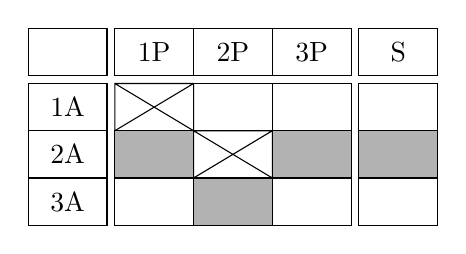
\begin{tikzpicture}[xscale=1, yscale=-.6, draw=black, fill=black!30]
	\draw     (-.1,-.17) node{}   +(-.5,-.5) rectangle ++(.5,.5);
	\draw     (1,-.17)   node{1P} +(-.5,-.5) rectangle ++(.5,.5);
	\draw     (2,-.17)   node{2P} +(-.5,-.5) rectangle ++(.5,.5);
	\draw     (3,-.17)   node{3P} +(-.5,-.5) rectangle ++(.5,.5);
	\draw     (4.1,-.17) node{S}  +(-.5,-.5) rectangle ++(.5,.5);
	\draw     (-.1,1)    node{1A} +(-.5,-.5) rectangle ++(.5,.5);
	\draw     (1,1)      node{}   +(-.5,-.5) rectangle ++(.5,.5) -- ++(-1,-1) ++(0,1) -- ++(1,-1);
	\draw     (2,1)      node{}   +(-.5,-.5) rectangle ++(.5,.5);
	\draw     (3,1)      node{}   +(-.5,-.5) rectangle ++(.5,.5);
	\draw     (4.1,1)    node{}   +(-.5,-.5) rectangle ++(.5,.5);
	\draw     (-.1,2)    node{2A} +(-.5,-.5) rectangle ++(.5,.5);
	\filldraw (1,2)      node{}   +(-.5,-.5) rectangle ++(.5,.5);
	\draw     (2,2)      node{}   +(-.5,-.5) rectangle ++(.5,.5) -- ++(-1,-1) ++(0,1) -- ++(1,-1);
	\filldraw (3,2)      node{}   +(-.5,-.5) rectangle ++(.5,.5);
	\filldraw (4.1,2)    node{}   +(-.5,-.5) rectangle ++(.5,.5);
	\draw     (-.1,3)    node{3A} +(-.5,-.5) rectangle ++(.5,.5);
	\draw     (1,3)      node{}   +(-.5,-.5) rectangle ++(.5,.5);
	\filldraw (2,3)      node{}   +(-.5,-.5) rectangle ++(.5,.5);
	\draw     (3,3)      node{}   +(-.5,-.5) rectangle ++(.5,.5);
	\draw     (4.1,3)    node{}   +(-.5,-.5) rectangle ++(.5,.5);
\end{tikzpicture}\\
\emph{-ka} \rede{2} (neutral, except 1>2)
\end{minipage}
\begin{minipage}[t]{.4\textwidth}
\centering
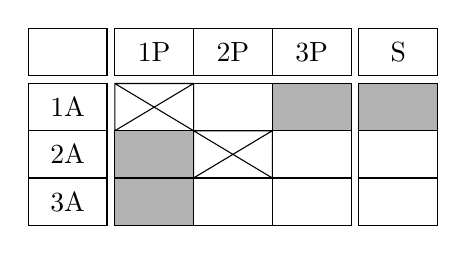
\begin{tikzpicture}[xscale=1, yscale=-.6, draw=black, fill=black!30]
	\draw     (-.1,-.17) node{}   +(-.5,-.5) rectangle ++(.5,.5);
	\draw     (1,-.17)   node{1P} +(-.5,-.5) rectangle ++(.5,.5);
	\draw     (2,-.17)   node{2P} +(-.5,-.5) rectangle ++(.5,.5);
	\draw     (3,-.17)   node{3P} +(-.5,-.5) rectangle ++(.5,.5);
	\draw     (4.1,-.17) node{S}  +(-.5,-.5) rectangle ++(.5,.5);
	\draw     (-.1,1)    node{1A} +(-.5,-.5) rectangle ++(.5,.5);
	\draw     (1,1)      node{}   +(-.5,-.5) rectangle ++(.5,.5) -- ++(-1,-1) ++(0,1) -- ++(1,-1);
	\draw     (2,1)      node{}   +(-.5,-.5) rectangle ++(.5,.5);
	\filldraw (3,1)      node{}   +(-.5,-.5) rectangle ++(.5,.5);
	\filldraw (4.1,1)    node{}   +(-.5,-.5) rectangle ++(.5,.5);
	\draw     (-.1,2)    node{2A} +(-.5,-.5) rectangle ++(.5,.5);
	\filldraw (1,2)      node{}   +(-.5,-.5) rectangle ++(.5,.5);
	\draw     (2,2)      node{}   +(-.5,-.5) rectangle ++(.5,.5) -- ++(-1,-1) ++(0,1) -- ++(1,-1);
	\draw     (3,2)      node{}   +(-.5,-.5) rectangle ++(.5,.5);
	\draw     (4.1,2)    node{}   +(-.5,-.5) rectangle ++(.5,.5);
	\draw     (-.1,3)    node{3A} +(-.5,-.5) rectangle ++(.5,.5);
	\filldraw (1,3)      node{}   +(-.5,-.5) rectangle ++(.5,.5);
	\draw     (2,3)      node{}   +(-.5,-.5) rectangle ++(.5,.5);
	\draw     (3,3)      node{}   +(-.5,-.5) rectangle ++(.5,.5);
	\draw     (4.1,3)    node{}   +(-.5,-.5) rectangle ++(.5,.5);
\end{tikzpicture}\\
\emph{-ŋ(a)} \rede{excl, 1sg} (neutral, except 1>2)
\end{minipage}\\[1em]

\begin{minipage}[t]{.4\textwidth}
\centering
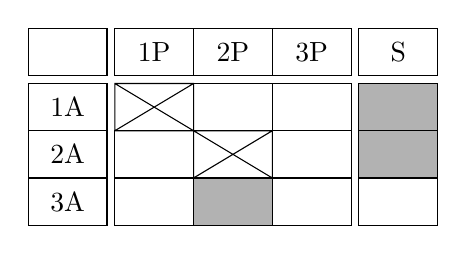
\begin{tikzpicture}[xscale=1, yscale=-.6, draw=black, fill=black!30]
	\draw     (-.1,-.17) node{}   +(-.5,-.5) rectangle ++(.5,.5);
	\draw     (1,-.17)   node{1P} +(-.5,-.5) rectangle ++(.5,.5);
	\draw     (2,-.17)   node{2P} +(-.5,-.5) rectangle ++(.5,.5);
	\draw     (3,-.17)   node{3P} +(-.5,-.5) rectangle ++(.5,.5);
	\draw     (4.1,-.17) node{S}  +(-.5,-.5) rectangle ++(.5,.5);
	\draw     (-.1,1)    node{1A} +(-.5,-.5) rectangle ++(.5,.5);
	\draw     (1,1)      node{}   +(-.5,-.5) rectangle ++(.5,.5) -- ++(-1,-1) ++(0,1) -- ++(1,-1);
	\draw     (2,1)      node{}   +(-.5,-.5) rectangle ++(.5,.5);
	\draw     (3,1)      node{}   +(-.5,-.5) rectangle ++(.5,.5);
	\filldraw (4.1,1)    node{}   +(-.5,-.5) rectangle ++(.5,.5);
	\draw     (-.1,2)    node{2A} +(-.5,-.5) rectangle ++(.5,.5);
	\draw     (1,2)      node{}   +(-.5,-.5) rectangle ++(.5,.5);
	\draw     (2,2)      node{}   +(-.5,-.5) rectangle ++(.5,.5) -- ++(-1,-1) ++(0,1) -- ++(1,-1);
	\draw     (3,2)      node{}   +(-.5,-.5) rectangle ++(.5,.5);
	\filldraw (4.1,2)    node{}   +(-.5,-.5) rectangle ++(.5,.5);
	\draw     (-.1,3)    node{3A} +(-.5,-.5) rectangle ++(.5,.5);
	\draw     (1,3)      node{}   +(-.5,-.5) rectangle ++(.5,.5);
	\filldraw (2,3)      node{}   +(-.5,-.5) rectangle ++(.5,.5);
	\draw     (3,3)      node{}   +(-.5,-.5) rectangle ++(.5,.5);
	\draw     (4.1,3)    node{}   +(-.5,-.5) rectangle ++(.5,.5);
\end{tikzpicture}\\
\emph{-i} \rede{1/2pl.S} \& \rede{2P}  (ergative for 2, except 1>2)
\end{minipage}
\begin{minipage}[t]{.4\textwidth}
\centering
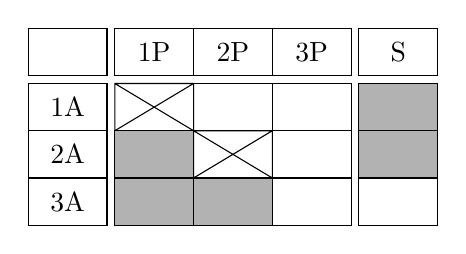
\begin{tikzpicture}[xscale=1, yscale=-.6, draw=black, fill=black!30]
	\draw     (-.1,-.17) node{}   +(-.5,-.5) rectangle ++(.5,.5);
	\draw     (1,-.17)   node{1P} +(-.5,-.5) rectangle ++(.5,.5);
	\draw     (2,-.17)   node{2P} +(-.5,-.5) rectangle ++(.5,.5);
	\draw     (3,-.17)   node{3P} +(-.5,-.5) rectangle ++(.5,.5);
	\draw     (4.1,-.17) node{S}  +(-.5,-.5) rectangle ++(.5,.5);
	\draw     (-.1,1)    node{1A} +(-.5,-.5) rectangle ++(.5,.5);
	\draw     (1,1)      node{}   +(-.5,-.5) rectangle ++(.5,.5) -- ++(-1,-1) ++(0,1) -- ++(1,-1);
	\draw     (2,1)      node{}   +(-.5,-.5) rectangle ++(.5,.5);
	\draw     (3,1)      node{}   +(-.5,-.5) rectangle ++(.5,.5);
	\filldraw (4.1,1)    node{}   +(-.5,-.5) rectangle ++(.5,.5);
	\draw     (-.1,2)    node{2A} +(-.5,-.5) rectangle ++(.5,.5);
	\filldraw (1,2)      node{}   +(-.5,-.5) rectangle ++(.5,.5);
	\draw     (2,2)      node{}   +(-.5,-.5) rectangle ++(.5,.5) -- ++(-1,-1) ++(0,1) -- ++(1,-1);
	\draw     (3,2)      node{}   +(-.5,-.5) rectangle ++(.5,.5);
	\filldraw (4.1,2)    node{}   +(-.5,-.5) rectangle ++(.5,.5);
	\draw     (-.1,3)    node{3A} +(-.5,-.5) rectangle ++(.5,.5);
	\filldraw (1,3)      node{}   +(-.5,-.5) rectangle ++(.5,.5);
	\filldraw (2,3)      node{}   +(-.5,-.5) rectangle ++(.5,.5);
	\draw     (3,3)      node{}   +(-.5,-.5) rectangle ++(.5,.5);
	\draw     (4.1,3)    node{}   +(-.5,-.5) rectangle ++(.5,.5);
\end{tikzpicture}\\
Historical forms (recent loss of 1nsg.P forms): \emph{-i} \rede{1/2pl.S/P} (ergative)
\end{minipage}\\[1em]

\begin{minipage}[t]{.4\textwidth}
\centering
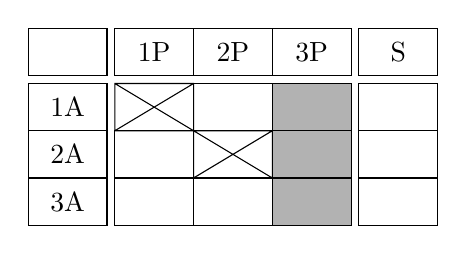
\begin{tikzpicture}[xscale=1, yscale=-.6, draw=black, fill=black!30]
	\draw     (-.1,-.17) node{}   +(-.5,-.5) rectangle ++(.5,.5);
	\draw     (1,-.17)   node{1P} +(-.5,-.5) rectangle ++(.5,.5);
	\draw     (2,-.17)   node{2P} +(-.5,-.5) rectangle ++(.5,.5);
	\draw     (3,-.17)   node{3P} +(-.5,-.5) rectangle ++(.5,.5);
	\draw     (4.1,-.17) node{S}  +(-.5,-.5) rectangle ++(.5,.5);
	\draw     (-.1,1)    node{1A} +(-.5,-.5) rectangle ++(.5,.5);
	\draw     (1,1)      node{}   +(-.5,-.5) rectangle ++(.5,.5) -- ++(-1,-1) ++(0,1) -- ++(1,-1);
	\draw     (2,1)      node{}   +(-.5,-.5) rectangle ++(.5,.5);
	\filldraw (3,1)      node{}   +(-.5,-.5) rectangle ++(.5,.5);
	\draw     (4.1,1)    node{}   +(-.5,-.5) rectangle ++(.5,.5);
	\draw     (-.1,2)    node{2A} +(-.5,-.5) rectangle ++(.5,.5);
	\draw     (1,2)      node{}   +(-.5,-.5) rectangle ++(.5,.5);
	\draw     (2,2)      node{}   +(-.5,-.5) rectangle ++(.5,.5) -- ++(-1,-1) ++(0,1) -- ++(1,-1);
	\filldraw (3,2)      node{}   +(-.5,-.5) rectangle ++(.5,.5);
	\draw     (4.1,2)    node{}   +(-.5,-.5) rectangle ++(.5,.5);
	\draw     (-.1,3)    node{3A} +(-.5,-.5) rectangle ++(.5,.5);
	\draw     (1,3)      node{}   +(-.5,-.5) rectangle ++(.5,.5);
	\draw     (2,3)      node{}   +(-.5,-.5) rectangle ++(.5,.5);
	\filldraw (3,3)      node{}   +(-.5,-.5) rectangle ++(.5,.5);
	\draw     (4.1,3)    node{}   +(-.5,-.5) rectangle ++(.5,.5);
\end{tikzpicture}\\
\emph{-u} \rede{3P}, \emph{-ci} \rede{3nsg.P}  (accusative)
\end{minipage}
\begin{minipage}[t]{.4\textwidth}
\centering
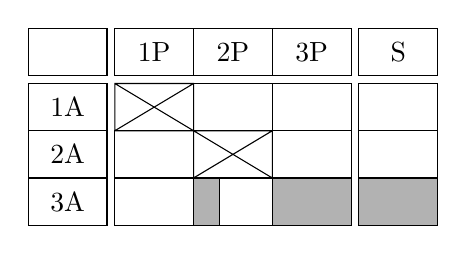
\begin{tikzpicture}[xscale=1, yscale=-.6, draw=black, fill=black!30]
	\draw     (-.1,-.17) node{}   ++(-.5,-.5) rectangle ++(1,1);
	\draw     (1,-.17)   node{1P} ++(-.5,-.5) rectangle ++(1,1);
	\draw     (2,-.17)   node{2P} ++(-.5,-.5) rectangle ++(1,1);
	\draw     (3,-.17)   node{3P} ++(-.5,-.5) rectangle ++(1,1);
	\draw     (4.1,-.17) node{S}  ++(-.5,-.5) rectangle ++(1,1);
	\draw     (-.1,1)    node{1A} ++(-.5,-.5) rectangle ++(1,1);
	\draw     (1,1)      node{}   ++(-.5,-.5) rectangle ++(1,1) -- ++(-1,-1) ++(0,1) -- ++(1,-1);
	\draw     (2,1)      node{}   ++(-.5,-.5) rectangle ++(1,1);
	\draw     (3,1)      node{}   ++(-.5,-.5) rectangle ++(1,1);
	\draw     (4.1,1)    node{}   ++(-.5,-.5) rectangle ++(1,1);
	\draw     (-.1,2)    node{2A} ++(-.5,-.5) rectangle ++(1,1);
	\draw     (1,2)      node{}   ++(-.5,-.5) rectangle ++(1,1);
	\draw     (2,2)      node{}   ++(-.5,-.5) rectangle ++(1,1) -- ++(-1,-1) ++(0,1) -- ++(1,-1);
	\draw     (3,2)      node{}   ++(-.5,-.5) rectangle ++(1,1);
	\draw     (4.1,2)    node{}   ++(-.5,-.5) rectangle ++(1,1);
	\draw     (-.1,3)    node{3A} ++(-.5,-.5) rectangle ++(1,1);
	\draw     (1,3)      node{}   ++(-.5,-.5) rectangle ++(1,1);
	\draw     (2,3)      node{}   ++(-.5,-.5) rectangle ++(1,1);
	\filldraw (3,3)      node{}   ++(-.5,-.5) rectangle ++(1,1);
	\filldraw (4.1,3)    node{}   ++(-.5,-.5) rectangle ++(1,1);
	%geteilt
	\filldraw (2,3)      node{}   ++(-.5,-.5) rectangle ++(.33,1);
\end{tikzpicture}\\
\emph{N-} \rede{3pl.S/A}, zero \rede{3sg.S/A} (accusative)
\end{minipage}\\[1em]

\begin{minipage}[t]{.4\textwidth}
\centering
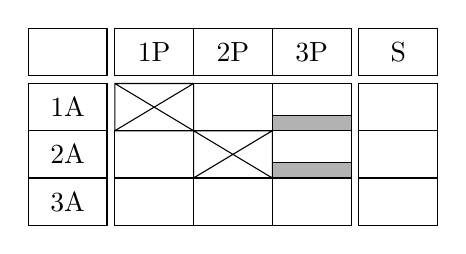
\begin{tikzpicture}[xscale=1, yscale=-.6, draw=black, fill=black!30]
	\draw     (-.1,-.17) node{}   ++(-.5,-.5) rectangle ++(1,1);
	\draw     (1,-.17)   node{1P} ++(-.5,-.5) rectangle ++(1,1);
	\draw     (2,-.17)   node{2P} ++(-.5,-.5) rectangle ++(1,1);
	\draw     (3,-.17)   node{3P} ++(-.5,-.5) rectangle ++(1,1);
	\draw     (4.1,-.17) node{S}  ++(-.5,-.5) rectangle ++(1,1);
	\draw     (-.1,1)    node{1A} ++(-.5,-.5) rectangle ++(1,1);
	\draw     (1,1)      node{}   ++(-.5,-.5) rectangle ++(1,1) -- ++(-1,-1) ++(0,1) -- ++(1,-1);
	\draw     (2,1)      node{}   ++(-.5,-.5) rectangle ++(1,1);
	\draw     (3,1)      node{}   ++(-.5,-.5) rectangle ++(1,1);
	\draw     (4.1,1)    node{}   ++(-.5,-.5) rectangle ++(1,1);
	\draw     (-.1,2)    node{2A} ++(-.5,-.5) rectangle ++(1,1);
	\draw     (1,2)      node{}   ++(-.5,-.5) rectangle ++(1,1);
	\draw     (2,2)      node{}   ++(-.5,-.5) rectangle ++(1,1) -- ++(-1,-1) ++(0,1) -- ++(1,-1);
	\draw     (3,2)      node{}   ++(-.5,-.5) rectangle ++(1,1);
	\draw     (4.1,2)    node{}   ++(-.5,-.5) rectangle ++(1,1);
	\draw     (-.1,3)    node{3A} ++(-.5,-.5) rectangle ++(1,1);
	\draw     (1,3)      node{}   ++(-.5,-.5) rectangle ++(1,1);
	\draw     (2,3)      node{}   ++(-.5,-.5) rectangle ++(1,1);
	\draw     (3,3)      node{}   ++(-.5,-.5) rectangle ++(1,1);
	\draw     (4.1,3)    node{}   ++(-.5,-.5) rectangle ++(1,1);
	%geteilt
	\filldraw (3,1)      node{}   ++(-.5,.5) rectangle ++(1,-.33);
	\filldraw (3,2)      node{}   ++(-.5,.5) rectangle ++(1,-.33);
\end{tikzpicture}\\
\emph{-m} \rede{1/2pl>3} (scenario-portmanteau)
\end{minipage}
\begin{minipage}[t]{.4\textwidth}
\centering
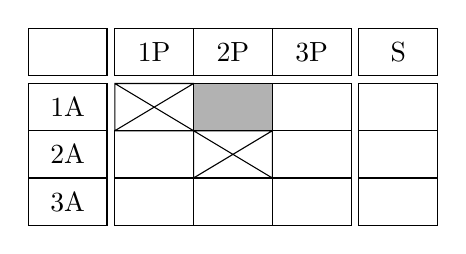
\begin{tikzpicture}[xscale=1, yscale=-.6, draw=black, fill=black!30]
	\draw     (-.1,-.17) node{}   ++(-.5,-.5) rectangle ++(1,1);
	\draw     (1,-.17)   node{1P} ++(-.5,-.5) rectangle ++(1,1);
	\draw     (2,-.17)   node{2P} ++(-.5,-.5) rectangle ++(1,1);
	\draw     (3,-.17)   node{3P} ++(-.5,-.5) rectangle ++(1,1);
	\draw     (4.1,-.17) node{S}  ++(-.5,-.5) rectangle ++(1,1);
	\draw     (-.1,1)    node{1A} ++(-.5,-.5) rectangle ++(1,1);
	\draw     (1,1)      node{}   ++(-.5,-.5) rectangle ++(1,1) -- ++(-1,-1) ++(0,1) -- ++(1,-1);
	\filldraw (2,1)      node{}   ++(-.5,-.5) rectangle ++(1,1);
	\draw     (3,1)      node{}   ++(-.5,-.5) rectangle ++(1,1);
	\draw     (4.1,1)    node{}   ++(-.5,-.5) rectangle ++(1,1);
	\draw     (-.1,2)    node{2A} ++(-.5,-.5) rectangle ++(1,1);
	\draw     (1,2)      node{}   ++(-.5,-.5) rectangle ++(1,1);
	\draw     (2,2)      node{}   ++(-.5,-.5) rectangle ++(1,1) -- ++(-1,-1) ++(0,1) -- ++(1,-1);
	\draw     (3,2)      node{}   ++(-.5,-.5) rectangle ++(1,1);
	\draw     (4.1,2)    node{}   ++(-.5,-.5) rectangle ++(1,1);
	\draw     (-.1,3)    node{3A} ++(-.5,-.5) rectangle ++(1,1);
	\draw     (1,3)      node{}   ++(-.5,-.5) rectangle ++(1,1);
	\draw     (2,3)      node{}   ++(-.5,-.5) rectangle ++(1,1);
	\draw     (3,3)      node{}   ++(-.5,-.5) rectangle ++(1,1);
	\draw     (4.1,3)    node{}   ++(-.5,-.5) rectangle ++(1,1);
\end{tikzpicture}\\
\emph{-nen} \rede{1>2} (scenario-portmanteau)
\end{minipage}\\[1em]

\begin{minipage}[t]{.4\textwidth}
\centering
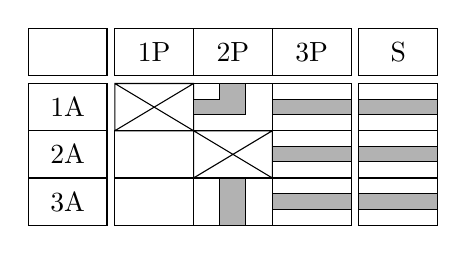
\begin{tikzpicture}[xscale=1, yscale=-.6, draw=black, fill=black!30]
	\draw     (-.1,-.17) node{}   ++(-.5,-.5) rectangle ++(1,1);
	\draw     (1,-.17)   node{1P} ++(-.5,-.5) rectangle ++(1,1);
	\draw     (2,-.17)   node{2P} ++(-.5,-.5) rectangle ++(1,1);
	\draw     (3,-.17)   node{3P} ++(-.5,-.5) rectangle ++(1,1);
	\draw     (4.1,-.17) node{S}  ++(-.5,-.5) rectangle ++(1,1);
	\draw     (-.1,1)    node{1A} ++(-.5,-.5) rectangle ++(1,1);
	\draw     (1,1)      node{}   ++(-.5,-.5) rectangle ++(1,1) -- ++(-1,-1) ++(0,1) -- ++(1,-1);
	\draw     (2,1)      node{}   ++(-.5,-.5) rectangle ++(1,1);
	\draw     (3,1)      node{}   ++(-.5,-.5) rectangle ++(1,1);
	\draw     (4.1,1)    node{}   ++(-.5,-.5) rectangle ++(1,1);
	\draw     (-.1,2)    node{2A} ++(-.5,-.5) rectangle ++(1,1);
	\draw     (1,2)      node{}   ++(-.5,-.5) rectangle ++(1,1);
	\draw     (2,2)      node{}   ++(-.5,-.5) rectangle ++(1,1) -- ++(-1,-1) ++(0,1) -- ++(1,-1);
	\draw     (3,2)      node{}   ++(-.5,-.5) rectangle ++(1,1);
	\draw     (4.1,2)    node{}   ++(-.5,-.5) rectangle ++(1,1);
	\draw     (-.1,3)    node{3A} ++(-.5,-.5) rectangle ++(1,1);
	\draw     (1,3)      node{}   ++(-.5,-.5) rectangle ++(1,1);
	\draw     (2,3)      node{}   ++(-.5,-.5) rectangle ++(1,1);
	\draw     (3,3)      node{}   ++(-.5,-.5) rectangle ++(1,1);
	\draw     (4.1,3)    node{}   ++(-.5,-.5) rectangle ++(1,1);
	%geteilt
	\filldraw (2,1)      ++(-.5,-.5) ++(.33,0)--++(.33,0)--++(0,.66)--++(-.66,0)--++(0,-.33)--++(.33,0)--++(0,-.33);
	\filldraw (3,1)      ++(-.5,-.5) ++(0,.33) rectangle ++(1,.33);
	\filldraw (4.1,1)    ++(-.5,-.5) ++(0,.33) rectangle ++(1,.33);
	\filldraw (3,2)      ++(-.5,-.5) ++(0,.33) rectangle ++(1,.33);
	\filldraw (4.1,2)    ++(-.5,-.5) ++(0,.33) rectangle ++(1,.33);
	\filldraw (3,3)      ++(-.5,-.5) ++(0,.33) rectangle ++(1,.33);
	\filldraw (4.1,3)    ++(-.5,-.5) ++(0,.33) rectangle ++(1,.33);
	\filldraw (2,3)      ++(-.5,-.5) ++(.33,0) rectangle ++(.33,1);
\end{tikzpicture}\\
\emph{-ci} \rede{dual} (mixed: acc./neutral/ref.-based)
\end{minipage}
\begin{minipage}[t]{.4\textwidth}
\centering
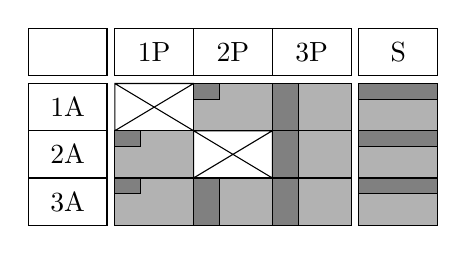
\begin{tikzpicture}[xscale=1, yscale=-.6, draw=black, fill=black!30]
	\draw     (-.1,-.17) node{}   ++(-.5,-.5) rectangle ++(1,1);
	\draw     (1,-.17)   node{1P} ++(-.5,-.5) rectangle ++(1,1);
	\draw     (2,-.17)   node{2P} ++(-.5,-.5) rectangle ++(1,1);
	\draw     (3,-.17)   node{3P} ++(-.5,-.5) rectangle ++(1,1);
	\draw     (4.1,-.17) node{S}  ++(-.5,-.5) rectangle ++(1,1);
	\draw     (-.1,1)    node{1A} ++(-.5,-.5) rectangle ++(1,1);
	\draw     (1,1)      node{}   ++(-.5,-.5) rectangle ++(1,1) -- ++(-1,-1) ++(0,1) -- ++(1,-1);
	\filldraw (2,1)      node{}   ++(-.5,-.5) rectangle ++(1,1);
	\filldraw (3,1)      node{}   ++(-.5,-.5) rectangle ++(1,1);
	\filldraw (4.1,1)    node{}   ++(-.5,-.5) rectangle ++(1,1);
	\draw     (-.1,2)    node{2A} ++(-.5,-.5) rectangle ++(1,1);
	\filldraw (1,2)      node{}   ++(-.5,-.5) rectangle ++(1,1);
	\draw     (2,2)      node{}   ++(-.5,-.5) rectangle ++(1,1) -- ++(-1,-1) ++(0,1) -- ++(1,-1);
	\filldraw (3,2)      node{}   ++(-.5,-.5) rectangle ++(1,1);
	\filldraw (4.1,2)    node{}   ++(-.5,-.5) rectangle ++(1,1);
	\draw     (-.1,3)    node{3A} ++(-.5,-.5) rectangle ++(1,1);
	\filldraw (1,3)      node{}   ++(-.5,-.5) rectangle ++(1,1);
	\filldraw (2,3)      node{}   ++(-.5,-.5) rectangle ++(1,1);
	\filldraw (3,3)      node{}   ++(-.5,-.5) rectangle ++(1,1);
	\filldraw (4.1,3)    node{}   ++(-.5,-.5) rectangle ++(1,1);
	%entspricht =na (in hellerem Grau)
	\begin{scope}[fill=black!50]
	\filldraw (2,1)      ++(-.5,-.5) rectangle ++(.33,.33);
	\filldraw (1,2)      ++(-.5,-.5) rectangle ++(.33,.33);
	\filldraw (1,3)      ++(-.5,-.5) rectangle ++(.33,.33);
	\filldraw (3,1)      ++(-.5,-.5) rectangle ++(.33,1);
	\filldraw (3,2)      ++(-.5,-.5) rectangle ++(.33,1);
	\filldraw (3,3)      ++(-.5,-.5) rectangle ++(.33,1);
	\filldraw (2,3)      ++(-.5,-.5) rectangle ++(.33,1);
	\filldraw (4.1,1)    ++(-.5,-.5) rectangle ++(1,.33);
	\filldraw (4.1,2)    ++(-.5,-.5) rectangle ++(1,.33);
	\filldraw (4.1,3)    ++(-.5,-.5) rectangle ++(1,.33);
	\end{scope}
\end{tikzpicture}\\
\emph{=na} \rede{sg}; \emph{=ha} \rede{nsg} (mixed: erg./ref.-based)
\end{minipage}
\caption{The alignment of individual person/number markers}\label{aligntables}
\end{figure}




%\end{document}



\section{Polarity}\label{neg}

There are two sets of \isi{negation} markers, one for nonfinite forms like converbs, participant nominalizations and infinitives, and one for finite inflected verbs. The first set is instantiated by the prefix \emph{men-}. 

In finite verbs, \isi{negation} is marked by an underspecified nasal prefix and a suffix (\emph{N-...-n}). In forms with {\scshape 3pl.A} and with {\scshape 1pl.incl.A}, \emph{-n} has the allomorph \emph{-nin}.\footnote{This allomorph has a slightly larger distribution in the inflection of the copulas, see  §\ref{cop-infl}.} By means of  \isi{nasal copying} \emph{-n} can occur up to three times in one inflected form (see \Next[a]). Comparing this form to \Next[b], one can see that \emph{-n} has replaced \emph{-ŋ} in the copy slots; now it is the \isi{negation} suffix that is copied. There is a hierarchy for the choice of which suffix to copy, consistently followed throughout the paradigms: \emph{-m > -n > -ŋ} (see also §\ref{sec-nasalcop}). 

\ex.\ag.n-chim-me-n-cu-n-ci-ŋa-n=ha\\
{\scshape neg-}ask{\scshape -npst-[copy]-du-3.P-[copy]-3nsg.P-excl-neg=nmlz.nsg}\\
	\rede{We (dual, excl.) will not ask them.}
	\bg. chim-me-ŋ-c-u-ŋ-ci-ŋ=ha\\
	ask{\scshape -npst-[copy]-du-3.P-N-3nsg.P-excl=nmlz.nsg}\\
	\rede{We (dual, excl.) will ask them.}
	
	
The unspecified nasal prefix assimilates in place to the first consonant of the verbal stem, as has been shown above for the nasal prefix coding third person plural subjects. For some forms, especially in the forms for first person acting on the second person, it is the only \isi{negation} marking device (see \Next). Among related languages, only Belhare has this unspecified nasal prefix, too \citep[554]{Bickel2003Belhare}. 

\ex. \ag.  chim-meʔ-nen=na\\
	 ask{\scshape -npst-1>2=nmlz.sg}\\
	\rede{I will ask you.}
		\bg.n-chim-meʔ-nen=na\\
	{\scshape neg-}ask{\scshape -npst-1>2=nmlz.sg}\\
	\rede{I will not ask you.}

	
Examples of the suffix \emph{-nin} are provided in \Next. As a \isi{comparison} between \Next[a] and \Next[b] shows, it may trigger the \isi{nasal copying} too, if no higher ranking nasal suffix is available. In forms with third person plural agents, the homophony between \emph{N-} marking person and \emph{N-} marking \isi{negation} makes this prefix ambiguous in these particular forms. Functionally, it would make sense to say that the task of \emph{-nin} is to disambiguate between affirmative and negative in those forms. But for the forms coding {\scshape 1pl>3} this explanation does not make sense. 
 
 \ex. \ag.n-chimd-wa-m-ci-m-nin=ha\\
			{\scshape neg-}ask{\scshape -npst-[copy]-3nsg.P-1pl.A-neg=nmlz.nsg}\\
		\rede{We (incl.) will not ask them.}
 	\bg.n-chimd-wa-n-ci-nin=ha\\
		{\scshape neg/3pl.A-}ask{\scshape -npst-[copy]-3nsg.P-neg=nmlz.nsg}\\
		\rede{They will not ask them.}
		
Paradigm tables can be found in §\ref{paradigmtables}, with the upper forms showing the affirmative and the lower forms showing the negative inflections. 	


\section{Tense and \isi{aspect} marking }\label{tense}

The inflected verb is marked  for \isi{tense} in both the indicative and the subjunctive \isi{mood}. Tensed forms stand in opposition to the non-tensed \isi{imperative }\isi{mood}. This section only treats \isi{tense} and \isi{aspect} in the indicative \isi{mood}, where \isi{tense} also shows more elaborate distinctions. The subjunctive is treated below in §\ref{mood}.

The basic distinction in \isi{tense} marking is between nonpast and past \isi{tense}, partly cross-cut by aspectual distinctions (\isi{progressive} and \isi{continuative} \isi{aspect}, both expressed periphrastically). As predicates with inceptive semantics are quite wide\-spread in Yakkha (as in Belhare, cf. \citealt{Bickel1996Aspect}), past inflections often have a \rede{present} interpretation, referring to the inception of a state or event, e.g. \emph{tugama}  (hurt.{\scshape prf[3sg]}) \rede{it started to hurt/it hurts}). Another consequence of this is that nonpast marking often gets a future  or a general interpretation (i.e. not referring to a particular event, as in  the nonpast \emph{tuŋmeʔna} \rede{it will hurt/it generally hurts}). 

An overview of the \isi{tense}/\isi{aspect} distinctions and their markers is provided in Table \ref{ov-TA}. The relative simplicity of this overview is misleading, though, since further aspectual/Aktionsart distinctions, such as  specifications for \isi{telicity} and irreversibility, are indicated by  complex predication (see Chapter \ref{verb-verb}). The \isi{tense}/\isi{aspect} analysis and labels presented here have to be understood as tentative, since no in-depth analysis of the lexical semantics of the verbs has been undertaken yet.

\begin{table}[htp]
\begin{centering}
\begin{tabular}{ll}
\lsptoprule
{\bf {\scshape nonpast}}&{\bf {\scshape past}}\\
\midrule
		{\scshape nonpast}&{\scshape simple past} \\
\hskip1em	\emph{-meʔ}/&\hskip1em\emph{-a}\\
\hskip1em		\emph{-wa}&\\
\midrule
				&{\scshape perfect} \\
				&\hskip1em \emph{-ama \ti -imi}  \\
				&\hskip1em \emph{-uks}\\
\midrule
				&{\scshape past perfect}\\
				&\hskip1em	\emph{-amasa \ti -imisi} \\
				&\hskip1em\emph{-uksa}\\
\midrule
{\scshape progressive}&{\scshape progressive}\\
\hskip1em{\scshape inf + aux.}\emph{siʔ}.{\scshape npst}&\hskip1em{\scshape inf + aux.}\emph{siʔ}.{\scshape pst}\\
\midrule
{\scshape continuative}&{\scshape continuative}\\
\hskip1em{\scshape sim.cvb + aux.}\emph{kheʔ}.{\scshape npst}&\hskip1em{\scshape sim.cvb + aux.}\emph{kheʔ}.{\scshape pst}\\
\lspbottomrule
\end{tabular}\\
\caption{Tense and \isi{aspect} inflection}\label{ov-TA}
\end{centering}
\end{table}



\subsection{The Nonpast}\label{npst}

Yakkha overtly marks the nonpast in the indicative but not in the subjunctive. The nonpast is indicated by the two suppletive markers \emph{-meʔ} and \emph{-wa}, occurring in different slots of the verbal inflection. While  \emph{-meʔ} comes immediately after the stem and before the \isi{person marking} (Slot 1), \emph{-wa} follows the suffix \emph{-i} \rede{1/2pl} (Slot 6). 

Historically, both markers are function verbs that got further grammaticalized to \isi{tense} markers. They are different from function verbs in not triggering the double inflection that is found in complex predication, and also in not showing up in the citation forms, as function verbs generally do. The lexical verb \emph{wama} \rede{sit, stay, live} still exists in Yakkha, but \emph{meʔma} only exists with the stem \emph{met} and the meaning \rede{put around the waist}. In Belhare and \ili{Bantawa}, though, cognates with the meaning \rede{make, do, apply, cause} can be found  \citep{Bickel1997Dictionary, Doornenbal2009A-grammar}. The Yakkha causative marker \emph{-met} is also cognate to the nonpast marker, and in analogy to the stems and augments treated in §\ref{stem} above,  \emph{meʔ} originates in an unaugmented stem and \emph{met} is the corresponding augmented stem. The final /ʔ/ is often omitted (the omission being triggered by the following material), but it still has an impact on the following material: if \emph{-ka} follows \emph{-meʔ}, it does not get voiced, for instance. The sequence becomes [meka], not [mega], because more than one consonant stands between the vowels  in the underlying structure.


The distribution of these two allomorphs is not random, but grammatically conditioned (see Table \ref{par-npst-allo}). In the intransitive paradigm, mostly \emph{-meʔ} is found, except for first and second person plural, which take \emph{-wa}. The picture is slightly more complex in the transitive paradigm. Again, the more common allomorph is \emph{-meʔ}, but \emph{-wa} occurs in the forms of third person acting on second person plural (\rede{3>2pl}), and in the forms with a non-dual agent and a third person patient. Thus, the distribution of the markers can be seen as  a secondary device to mark different scenario classes, albeit not according to a particular referential hierarchy.  Example paradigms can be found in §\ref{paradigmtables}. 

As for the development of this system I can only speculate but it is worth mentioning that in Yakkha complex predication, some function verbs (V2s) are employed to specify the \isi{transitivity} features of a verb. It is possible that the historical V2 stems \emph{-meʔ} and \emph{-wa} have also been distributed according to \isi{transitivity} features, and that via this stage their distribution was re-arranged so that they became markers of participant scenarios.


\begin{table}
\begin{centering} 
\begin{tabular}{|l||l|p{1.4cm}|p{1.4cm}|l|p{1.4cm}|}
\hline
		& {\scshape intransitive}&	\multicolumn{4}{c|}{ {\scshape transitive}}  \\
		\cline{3-6}
		&&	 {\scshape 1}&  {\scshape 2}&  {\scshape 2pl} &  {\scshape 3} \\
\hline
\hline
 {\scshape 1sg} 		&-meʔ& \cellcolor[gray]{.8}&\multicolumn{2}{c|}{}&-wa\\
 \cline{1-1} \cline{6-6} 		
 {\scshape 1du}		& & \cellcolor[gray]{.8}&\multicolumn{2}{c|}{-meʔ}&-meʔ\\
 \cline{1-2} \cline{6-6} 			
 {\scshape 1pl}		&-wa & \cellcolor[gray]{.8}&\multicolumn{2}{c|}{}&-wa\\
 \cline{1-5}				
 {\scshape 2sg} 		&-meʔ &&\multicolumn{2}{c|}{\cellcolor[gray]{.8}} &\\
 \cline{1-1} \cline{6-6}			
 {\sc2du}		& &-meʔ& \multicolumn{2}{c|}{\cellcolor[gray]{.8}}  &-meʔ\\
 \cline{1-2} \cline{6-6}			
 {\sc2pl}		&-wa &&\multicolumn{2}{c|}{\cellcolor[gray]{.8}}  &-wa\\
 \cline{1-5}				
 {\scshape 3sg} 		&&\multicolumn{2}{c|}{} &  &\\
  \cline{1-1}  \cline{6-6}					
 {\scshape 3du}&-meʔ&\multicolumn{2}{c|}{-meʔ}  &  -wa&-meʔ\\
 \cline{1-1} \cline{6-6}
 {\scshape 3pl}& &\multicolumn{2}{c|}{}&  &-wa\\
\hline
\end{tabular}
\caption{Distribution of nonpast allomorphs}\label{par-npst-allo}
\end{centering}
\end{table}

Let us now turn to the functional distribution of the category nonpast. As mentioned above, verbs marked by the nonpast  often acquire a future reading (see \Next).  Furthermore, the nonpast is  found in general statements and in procedural texts, i.e. when the speaker does not have a particular temporal reference in mind (see \NNext). 

\ex.\ag.sombar=ŋa ta-meʔ=na\\
Monday{\scshape =ins} come{\scshape [3sg]-npst=nmlz.sg}\\
\rede{He will come on Monday.}
\bg.wandik=ŋa nam phem-meʔ=na\\
next\_day{\scshape =ins} sun shine{\scshape [3sg]-npst=nmlz.sg}\\
\rede{Tomorrow the sun will shine.}

\ex. \ag. nhaŋto, garo n-cheŋd-et-wa=na,      tokhaʔla\\
afterwards terrace {\scshape 3pl.A-}build{\scshape -V2.carry.off-npst=nmlz.sg} upwards\\
\rede{And then they build the terrace, upwards.}\footnote{The example is from a description of the  construction of houses, referring to the stabilization of terraced fields around the house by means of field stones.}  \source{31\_mat\_01.093}
\bg.panca=ci, bhaladmi=ci n-yuks-wa-ci=hoŋ  ceʔya n-jekt-wa,\\
an\_official\_rank{\scshape =nsg} respected\_elder{\scshape =nsg} {\scshape 3pl.A-}put{\scshape -npst-3nsg.P=seq} matter {\scshape 3pl.A-}talk{\scshape -npst}\\
\rede{They summon the officials and respected men, and they discuss the matter.} (a marriage description) \source{25\_tra\_01.008}

The nonpast is also possible in adverbial  clauses, such as sequential \Last[b], cotemporal or \isi{conditional clauses}, if the proposition is true or likely to become true (cf. Chapter \ref{adv-cl}). 

\subsection{The Past Tenses}\label{pst}

The past tenses stand in complementary distribution to each other (and to the nonpast). Yakkha has the simple past, the perfect, and the past perfect. Morphologically, the perfect is a specification of the simple past, and the past perfect is a specification of the perfect, since in each form, some morphological material is added (see Table \ref{ov-TA}).

\subsubsection{The simple past}\label{sim-pst}

The simple past is marked by \emph{-a}, in the same slot as \emph{-meʔ}. The two markers behave alike in preceding the second person marker \emph{-ka} and they never co-occur (see \Next). The suffix is homophonous with the \isi{imperative} and the Past Subjunctive (see §\ref{mood}), but ambiguities are resolved by context and partly by alternative person or \isi{negation} marking suffixes in the non-indicative moods.

\ex. \ag.  py-a-ga=na\\
			give{\scshape [3.A]-pst-2.P=nmlz.sg}\\
			\rede{He gave it to you.}
	\bg. pi-meʔ-ka=na\\ 
			give{\scshape [3.A]-pst-2.P=nmlz.sg}\\
			\rede{He gives it to you.}
			
As for the morphophonology of this marker, it may cause the insertion of \isi{glides} after vowels, as in \emph{uyana} /u-a=na/ \rede{he entered}, or \emph{tayana} /ta-a=na/ \rede{he came}. In CVʔ stems, it causes the elision of /ʔ/, and the stem vowels /i/ and /e/ become [y], resulting in forms like   \emph{khyana} /kheʔ-a=na/ \rede{he went} (see also \Last[a]).  When \emph{-a} precedes the third person patient marker \emph{-u}, the former gets deleted (see \Next[a]). The same happens when \emph{-a} precedes \emph{-i}, as in \Next[b]. If such sequences occur after an open stem or a CVʔ stem, both suffixes are deleted (see \Next[c] and (e)). Another pair illustrating these processes is shown in \NNext. In (a) both suffixes undergo elision; in (b), since only two vowels are adjacent, a glide is inserted.\footnote{In \ili{Puma}, a Kiranti language of the Southern Central branch, a similar vowel elision in the suffix string results in vowel lengthening and low tone \citep{Bickeletal2006The-Chintang}. For Yakkha, this could not be detected.} Interestingly, the underlying sequence /iʔ-a-i-/ is realized [iʔi], a sequence that is not found elsewhere in the language (cf. paradigm of \emph{piʔma} \rede{give} on page \pageref{par-pipma-pst}). For more on morphophonology see §\ref{morphophon}. Paradigms of past inflections are provided in §\ref{paradigmtables}.

\ex.\a.\glll chimd-u-ŋ=na\\
 /chimd-a-u-ŋ=na/\\
ask{\scshape -pst-3.P-1sg.A=nmlz.sg}\\
\rede{I asked him.}
\b.\glll khe-i=ha\\
 /kheʔ-a-i=ha/\\
go{\scshape -pst-1pl=nmlz.nsg}\\
\rede{We (incl.) went.}
\b.\glll ta-ŋ=na \\
/taʔ-a-u-ŋ=na/\\
bring{\scshape -pst-3.P-1sg.A=nmlz.sg}\\
\rede{I brought him.}
\b.\glll pi-ga=na \\
/piʔ-a-u-ga=na/\\
give{\scshape -pst-3.P-2.A=nmlz.sg}\\
\rede{You gave it to him.}

\ex. \a.\glll ca-m=na\\
 /ca-a-u-m=na/\\
eat{\scshape -pst-3.P-1pl.A=nmlz.sg}\\
\rede{We (plural) ate it.}
\b.\glll ca-ya-c-u=na \\
/ca-a-c-u=na/\\
eat{\scshape -pst-du-3.P=nmlz.sg}\\
\rede{We (dual) ate it.}


The simple past  refers to past events that are not specified further, for instance in truth value questions, such as  in inquiries about whether a certain event happened or not, illustrated by \Next. 

\ex. \ag.  cek-met-u-m-ci-m-ga=m,                                    n-jek-met-u-m-ci-m-ga-n=ha=m?\\
speak{\scshape -caus-3.P-N-3nsg.P-2pl.A-2=alt} {\scshape neg-}speak{\scshape -caus-3.P-N-3nsg.P-2pl.A-2-neg=nmlz.nsg=alt}\\
\rede{Did you make them speak or did you not?} (talking about prospective bride and groom) \source{36\_cvs\_06.323}
\bg. khokt-a-ga=na?\\
chop\_off{\scshape -pst-2.P=nmlz.sg}\\
\rede{Does it taste pungent?} \source{36\_cvs\_06.011}


As mentioned above, many verbs in Yakkha (and generally in Kiranti, \citet[512]{Ebert2003Kiranti}) have ingressive-\isi{phasal} Aktionsart, emphasizing the inception of the event, so that past inflection refers to the ongoing state or activity, e.g. in \Last[b]. A common expression is shown in \Next[a], also rendered as \rede{it's done} (Nep. \emph{bhayo}), the past suffix being hardly audible in fast speech. Another example of the numerous verbs with such a temporal profile is shown in \Next[b].

\ex.\ag.leks-a=ha [leksha]\\
become{\scshape [3sg]-pst=nmlz.nc}\\
\rede{That's it.}
\bg.o-pomma=ci ŋ-gy-a=ha=ci [ŋghyaci]\\
{\scshape 3sg.poss-}laziness{\scshape =nsg} {\scshape 3pl-}come\_up{\scshape -pst=nmlz.nsg=nsg}\\
\rede{He feels lazy.}

Habitual past statements can also be made using the simple past \Next. There is no dedicated marker or construction for habitual \isi{aspect} in Yakkha.

\exg. encho,        a-ppa             wa-ya=niŋa               lit-u-m-ŋa=ba\\
long\_ago {\scshape 1sg.poss-}father exist{\scshape [3]-pst=ctmp} plant{\scshape [pst]-3.P-1pl.A-excl=emph}\\
\rede{Long ago, when my father was still alive, we used to plant it.} \source{36\_cvs\_06.086}

In \Next, the simple past refers to iterative events of reaching various places, which is conveyed by the duplicated question word.

\exg.didi,        ŋkhoŋ    heʔne heʔne tas-u-ga=na                    laʔlo?\\
sister, afterwards where where reach{\scshape [pst]-3.P-2.A=nmlz.sg} {\scshape ctr.excla}\\
\rede{Sister, where have you been?/Sister, which places did you reach?}  \source{36\_cvs\_06.183}

The simple past indicative cannot be distinguished from the past subjunctive in most person configurations, and thus, it is often not clear whether adverbial clauses are in the indicative or in the subjunctive, as can well be perceived in \LLast. However, since other tenses like the present, the perfect and past perfect (discussed below) are also possible in certain adverbial clauses, I assume that the simple past is possible as well. 

Based on the past forms, two more tenses can be constructed, namely the perfect and the past perfect (discussed in the following sections). 

\subsubsection{The perfect}\label{prf}

Roughly, the perfect \isi{tense}, with the allomorphs \emph{-ma} and \emph{-uks}, marks events for the past, but with continuing relevance for  the time of the utterance, again with interpretations depending on the internal temporal structure of the verbs. In \Next[a] the verb has a telic structure, so that the perfect expresses the successful accomplishment, while in \Next[b] and \Next[c] the verbs have ingressive-\isi{phasal} semantics, so that the perfect expresses a state. In \Next[c], the function verb \rede{give} adds a semantic shade of completeness, translatable as \rede{already}, sometimes also as \rede{certainly, inevitably}.

\ex. \ag. nhaŋ    ca-ma,     i=ʔlo,   lop whaŋd-uks-u-ŋ-ci-ŋ\\
		and\_then eat{\scshape -inf[deont]} what{\scshape =excla} now boil{\scshape -prf-3.P-N-3nsg.P-1sg.A}\\
		\rede{And we have to eat them, I have just boiled them.} \source{36\_cvs\_06.037}
		\bg.lop sak=ŋa n-sy-ama-ŋa-n=na\\
now hunger{\scshape =ins} {\scshape neg-}die{\scshape -prf-1sg-neg=nmlz.sg}\\
		\rede{I am not hungry now.} (\rede{I did not get hungry.})
	\bg.u-laŋ=be yeb-a-by-ama=na\\
	{\scshape 3sg.poss-}foot{\scshape =loc} stand{\scshape [3sg]-pst-V2.give-prf=nmlz.sg}\\
	\rede{She became independent already.} (\rede{She already stands on her own feet.})
	
A typical constraint on the perfect crosslinguistically is that this \isi{tense} marking is not compatible with specifying events in the past (see \citep[176]{Bickel1996Aspect} for the same point on Belhare). In \Next, for instance, the \isi{adverb} \emph{asen} is part of the adverbial clause only. The main clause (\rede{... bad things have happened}) implies that the things that happened still bear a certain relevance for the present, which is true, because the speakers utter an excuse for their rude behavior in the previous night when they were drunk.

\exg.	kaniŋ asen      men-ni=nuŋ         men-ni=nuŋ=ca                isisi leks-a-ma=ha\\
{\scshape  1pl[erg]} yesterday {\scshape neg-}know{\scshape =com.cl} {\scshape neg-}know{\scshape =com.cl=add} ugly happen{\scshape [3sg]-pst-prf=nmlz.nc}\\
\rede{Even though we did not notice it yesterday, something bad has happened.} \source{41\_leg\_09.064}
	
Contrary to the statement that the perfect expresses events that still have a certain relevance for the present, this \isi{tense} form also figures prominently in narratives. It seems that this is a strategy to connect the content of the story told to the here and now of the uerance context and thus to make it more ‘real’ and create suspense. More research is needed to reveal the exact application of the perfect.

As for the conditions of the perfect allomorphy, in the intransitive inflection, the form marked by the simple past suffix \emph{-a} serves as base to which the suffix \emph{-ma} for the perfect is attached. In forms with the suffix \emph{-i}  (i.e., where \emph{-a} surfaces as [i]), the marker has an allomorph \emph{-mi}, i.e. the suffix \emph{-i} for  {\scshape 1/2pl} regressively influences the vowel quality of the two suffixes \emph{-a} and \emph{-ma} (see \Next). 

\ex.\ag.khy-a-ma-ci-ŋ=ha\\
go{\scshape -pst-prf-du-excl=nmlz.nsg}\\
\rede{We (dual) have gone.}
\bg.khe-i-mi-ŋ=ha\\
go{\scshape -1pl-prf-excl=nmlz.nsg}\\
\rede{We (plural) have gone.} 


In the transitive paradigm, a suppletive allomorph \emph{-uks \ti -nuŋ} (pre-vocalic vs. pre-consonantal alternants) comes into play. This allomorph never co-occurs with \emph{-a}. As has been shown above for the allomorphy of the nonpast markers, this allomorphy is conditioned by scenario classes, i.e. by participant configurations, albeit with a slightly different distribution than in the nonpast allomorphy. Again, it is  not possible to find one particular  principle or hierarchy triggering the allomorphy. The perfect allomorphy is less complex than the nonpast allomorphy: it partly indicates inverse vs. direct scenarios (with a 3>1, 3>2 and 2>1 scenarios being inverse and marked by \emph{-ma}), but it also indicates \isi{number} of the agent in all scenarios with a third person patient, since in those forms all dual agents trigger \emph{-ma}, while singular and plural agents trigger \emph{-uks}. In the suffix string, \emph{-uks \ti -nuŋ} shares Slot 1 with {\scshape npst} \emph{-meʔ} and   \emph{-a}, and \emph{-ma \ti -mi} follows  \emph{-a} (which surfaces as [i] in {\scshape  1/2pl} forms)  in Slot 2.

Table \ref{par-prf-allo} shows the distribution of the allomorphs across the inflectional paradigms (intransitive and transitive). Paradigm tables can be found on page \pageref{par-apma-pst} for the intransitive inflection and on page \pageref{par-chimd-prf} for the transitive inflection. 

\begin{table}
\begin{centering} 
%\begin{tabular}{|l||l|l|c|l|}
\begin{tabular}{|l||p{1.7cm}|p{1.5cm}|p{1.5cm}|p{1.5cm}|p{1.5cm}|}
\hline
		& {\scshape intransitive}&	\multicolumn{3}{c|}{ {\scshape transitive}}  \\
		\cline{3-5}
		&&	 {\scshape 1}&  {\scshape 2} & {\scshape  3} \\
\hline
\hline
 {\scshape 1sg} 		&& \cellcolor[gray]{.8}&&-uks \\
 \cline{1-1} \cline{5-5} 		
 {\scshape 1du}		& & \cellcolor[gray]{.8}&-nuŋ&-ma\\
 \cline{1-1} \cline{5-5} 			
 {\scshape 1pl}	&& \cellcolor[gray]{.8}&&-uks \\
 \cline{1-1}  \cline{3-4} 		
 {\scshape 2sg	}	& &&\cellcolor[gray]{.8} &   \\
 \cline{1-1} \cline{5-5}			
 {\scshape 2du}	&-ma &&\cellcolor[gray]{.8}  &-ma\\
 \cline{1-1} \cline{5-5}			
 {\scshape 2pl}	& &&\cellcolor[gray]{.8}   &-uks \\
\cline{1-1}  \cline{4-4} 
 {\scshape 3sg}		&&\multicolumn{2}{c|}{}  & \\
  \cline{1-1}  \cline{5-5}					
 {\scshape 3du}&&\multicolumn{2}{c|}{}  &-ma\\
 \cline{1-1} \cline{5-5}
 {\scshape 3pl}& &\multicolumn{2}{l|}{-ma}  &-uks \\
\hline
\end{tabular}
\caption{Distribution of perfect allomorphs}\label{par-prf-allo}
\end{centering}
\end{table}

The etymological sources of these markers are also function verbs. At least \emph{-uks} has the unmistakable structure of a verbal stem. Its lexical origin could either be the verb \emph{uks} \rede{come down} or \emph{yuks} \rede{put, keep}. The pre-consonantal variant \emph{-nuŋ} of \emph{-uks} is also reminiscent of morphophonological processes in complex predicates. The origin of \emph{-ma} could not be traced. These markers differ from function verbs   in not appearing in the infinitival forms (citation forms, for instance) and in not licensing the \isi{recursive inflection} that is typical for complex predication (cf. Chapter \ref{verb-verb}). 

	
\subsubsection{The past perfect}\label{pstprf}
	
The perfect marking, in turn, serves as base to which \emph{-sa \ti -si} is attached (\emph{-si} being triggered by suffix \emph{-i}, in analogy to the perfect allomorphy of \emph{-ma \ti -mi}). Thus, one arrives at the complex past perfect markers \emph{-amasa \ti -imisi} and  \emph{-uksa}, with the same distribution across the participant scenarios as found in the perfect. The suffix \emph{-sa} might be etymologically related to the past copular stem \emph{sa}. 

This \isi{tense} form expresses events that happened prior to another event that has been activated in discourse, as shown in \Next.

\ex. \ag.hakt-a-ŋ-ga-ni bhoŋ mit-amasa-ŋ=na\\
send{\scshape -sbjv-1sg.P-2.A-opt} {\scshape comp} think{\scshape -pst.prf-1sg=nmlz.sg}\\
\rede{I had hoped that you would send me something.} (said either after receiving a parcel or after realizing that nothing was sent)
\bg.heʔne khy-amasa-ga=na?\\
where go{\scshape -pst.prf-2=nmlz.sg}\\
\rede{Where had you gone?} (it was clear from the context that the person was on the way back to her village) 
	\bg.u-mik encho=ba homd-uksa=na, hensen=go nu-yama=na\\
		{\scshape 3sg.poss-}eye long\_ago{\scshape =emph} swell{\scshape -pst.prf=nmlz.sg} these\_days{\scshape =top} get\_well{\scshape -prf=nmlz.sg}\\
		\rede{His eye had been swollen before, but these days it got well.}
		
		
\subsection{The  progressive}\label{progressive}

The  \isi{progressive} is constructed from an infinitival form of the lexical verb and the auxiliary \emph{siʔ}, which can carry person markers and  either Present or  simple past inflection. This construction resembles infinitival complement constructions and has probably developed out of such a construction. But here, the two predicates are fused at a lower level. This is also reflected by the morphology and by \isi{stress assignment}, which treat the whole complex as one unit. The auxiliary, unlike matrix verbs in complement constructions, does not carry main stress; it forms one domain for \isi{stress assignment} with the lexical verb. The auxiliary does not have an infinitival form (in contrast to complement-taking verbs, which may appear in the \isi{infinitive} and thus be embedded recursively into other complements). Inflectional prefixes, which attach to the matrix verb in complement constructions, attach to the \isi{infinitive} of the lexical verb in the \isi{progressive} (compare \Next[a] with \Next[b] and (c)). This leads to the unusual situation of an \isi{infinitive} marker standing between the prefix and the suffixes of an inflected verb.\footnote{This construction is best characterized as a hybrid between synthetic and analytic (periphrastic) marking, since the auxiliary behaves like a verbal stem at least with regard to the suffixes it may host. Thus, it is not treated with regard to the slot analysis.} 


\ex. \ag. haku nda nhe uŋ-ma n-dokt-wa-ga-n=na\\
		from.now.on {\scshape 2sg} here come\_down{\scshape -inf} {\scshape neg-}get\_chance{\scshape -npst[3.P]-2sg.A-neg=nmlz.sg}	\\
	\rede{Now you will not get the chance to come down here any more.} \source{21\_nrr\_04.035}
 	\bg. nna  seʔni=ŋa       caleppa l-lem-ma-sy-a=ha\\ 
		that night{\scshape =ins} bread {\scshape 3pl-}fry{\scshape -inf-aux.prog-pst=nmlz.nc}\\
	\rede{That night they were frying bread.}  \source{40\_leg\_08.032}
	\bg. uŋ=ŋa   pyak sakheʔwa=ci=ŋa     casak ŋ-gom-ca-ma-sim-me=ha nis-uks-u-ci\\
 {\scshape 3sg=erg} many  pigeon{\scshape =nsg=erg} uncooked\_rice  {\scshape 3pl}-pick\_up{\scshape -V2.eat-inf-aux.prog-npst=nmlz.nsg} see{\scshape [3sg.A]-prf-3.P-3nsg.P}\\
\rede{He saw many pigeons who were picking up (pecking with their beaks) and eating the rice.} \source{01\_leg\_07.013}



Semantically, the \isi{progressive} generally marks events as ongoing at the point of speaking (present \isi{progressive}) or at a point prior to the speech situation (past \isi{progressive}). However, looking at \Last[c], it becomes clear that the speech situation is not the only possible temporal anchor for the present \isi{progressive}, since in this example, the  point of reference is the event denoted by the main verb \rede{see}, and the \isi{progressive} marking of the embedded clause has to be interpreted with respect to the main clause.


The \isi{progressive} is also commonly found in adverbial clauses with \emph{-niŋ}, the marker for the cotemporality of two linked clauses (see \Next). 

\exg.u-sa   sem-saŋ        u-sam=be               ca-ma-sy-a-ŋ=niŋ, \\
{\scshape 3sg.poss-}fruit pluck{\scshape -sim.cvb}  {\scshape 3sg.poss-}root{\scshape =loc} eat{\scshape -inf-aux.prog-pst-1sg=ctmp}\\
\rede{As I was plucking and eating the fruits under the tree, ...}\footnote{The noun \emph{sam} is a relational noun,  with the metaphorical meaning \rede{under/at the bottom of}.} \source{42\_leg\_10.017}

Interestingly, the \isi{progressive} auxiliary is sensitive to the speech-act-participant (SAP/non-SAP) distinction. It is inflected like an intransitive verb when  third person P arguments are involved, also when the semantic head is a transitive verb (see \Next[a]). The auxiliary verb shows  agreement with the S or the A of the lexical verb. A transitive example as in \LLast[c] also shows that despite the intransitive \isi{person marking}  the lexical verb is still able to assign the \isi{ergative} \isi{case} to the subject (\emph{sakheʔwaciŋa}).  When the object is a speech act participant, it shows transitive \isi{person marking}, as exemplified in \Next[b] and (c). This process is not surprising given the abundance of differential marking that is triggered by the referential properties of arguments in Yakkha.

\ex.\ag. ka kucuma yok-ma-si-me-ŋ=na\\
	{\scshape 1sg[erg]} dog search-{\scshape inf-aux.prog-npst-1sg=nmlz.sg}\\
	\rede{I am looking for the dog.}  (*\emph{yokmasiwaŋna})
\bg. ka nda yok-ma-si-meʔ-nen=na\\
{\scshape 1sg[erg]} {\scshape 2sg} search-{\scshape inf-aux.prog-npst-1>2=nmlz.sg}\\
\rede{I am looking for you.}	
\bg. phoʈo=ci soʔ-meʔ-ma-sy-a-ŋ-ga=na\\
photo{\scshape =nsg} look{\scshape -caus-inf-aux.prog-pst-1sg.P-2.A=nmlz.sg}\\
\rede{You were showing me the photos.}

\subsection{The periphrastic continuative}

This construction has developed out of a \isi{converb} construction, in analogy to a similar construction in \ili{Nepali}. The lexical head is marked by the converbal marker \emph{-saŋ} and the  main verb is invariably \emph{kheʔma} \rede{go}, but it has undergone \isi{grammaticalization} to an auxiliary, from \isi{motion} verb semantics to the expression of continuous events, similar to the English expression \rede{go on doing}. A formerly biclausal construction has become monoclausal.

The \isi{continuative} expresses that an event goes on over a longer stretch of time. It applies regardless of whether the verb has active, volitional semantics \Next[a] or rather change-of-state semantics (see \Next[b]). Example \Next[a] also shows that the auxiliary is compatible  with the perfect \isi{tense}. Example \Next[b] shows that in contrast to the periphrastic \isi{progressive}, prefixes attach to the auxiliary. In \Next[c], the construction is shown with a transitive lexical verb. The auxiliary is still inflected intransitively, showing agreement with the A argument of the lexical verb.  
 	
\ex.\ag. nakhaʔla   luk-khusa    ca-saŋ           khy-ama-ci=niŋa...\\
like\_that tell{\scshape -recip} {\scshape eat.aux-sim.cvb} go{\scshape -prf-du=ctmp}\\
\rede{As the two went on arguing (lit: with each other) like that, ...} \source{01\_leg\_07.340}
\bg.yapmi=ci pu-saŋ ŋ-khy-a\\
person{\scshape =nsg} grow{\scshape -sim.cvb}  {\scshape 3pl-}go{\scshape -pst}\\
\rede{The \isi{number} of the people grew continuously, ...} \source{27\_leg\_06.003}
 \bg.      iŋ-nhaŋ-saŋ            ik-saŋ         khy-a-ci=niŋa,\\
 chase{\scshape -V2.send-sim} chase{\scshape -sim} go{\scshape -pst-du=ctmp}\\
 \rede{As they (dual) went on chasing them away, ...} \source{22\_nrr\_05.015}
 
\subsection{The transitive completive}\label{completive}
 
 The marker  \emph{-i \ti -ni} for \isi{completive} events is only found in transitive verbs. It surfaces as [i] before vowels and as [ni] before consonants (see \Next and \NNext). 
 
 \ex.\ag.mend-i\\
 finish{\scshape -compl[3A;3P]}\\
 \rede{It is finished.}
 \bg.chimd-i-ŋ=na\\
ask{\scshape -compl[3P;pst]-1sg.A=nmlz.sg}\\
\rede{I finished asking him.}
 
The marker partly behaves like a function verb, and is thus not treated in the slot analysis (see also §\ref{V2-compl}): it precedes Slot 1 in the inflection, and it stands in complementary distribution with the V2 \emph{-piʔ} \rede{give}, which (among many other functions) indicates \isi{completive} notions in intransitive  predicates. The marker \emph{-i \ti -ni} also surfaces in the citation forms, like a function verb. There is, however, no lexical verb (at least not synchronically) that it relates to. The two markers often create lexicalized pairs of intransitive and causative verbs (see \Next, repeated from Chapter \ref{verb-verb}, where more examples can be found). Roots like \emph{maks}  never occur independently; either \emph{-i \ti -ni} or \emph{-piʔ} have to attach to them and specify their \isi{valency}. 

 
\ex. \ag.maŋmaŋ-miŋmiŋ m-maks-a-by-a-ma\\
	surprised{\scshape -redupl} {\scshape 3pl-}surprise{\scshape -pst-V2.give-pst-prf}\\
	\rede{They were utterly surprised.} \source{22\_nrr\_05.026}
 	\bg.ka nda mak-ni-meʔ-nen=na\\
	{\scshape 1sg[erg]} {\scshape 2sg[nom]} surprise{\scshape -compl-npst-1>2=nmlz.sg}		\\
	\rede{I will surprise you.} 
	

 
 
 
% \newpage
 
